\documentclass[11pt,a4paper]{article}
\usepackage[utf8]{inputenc}
\usepackage[english]{babel}
\usepackage[T1]{fontenc}
\usepackage{amsmath}
\usepackage{amsfonts}
\usepackage{amssymb}
\usepackage{makeidx}
\usepackage{graphicx}
\usepackage{hyperref}
\usepackage{placeins}
\usepackage{siunitx}
\usepackage{subcaption}
\usepackage[left=2cm,right=2cm,top=2cm,bottom=2cm]{geometry}

\usepackage{tikz}
\usetikzlibrary{arrows.meta,positioning,calc,shapes}
\usepackage{siunitx}
\setlength{\parindent}{0pt} 
\begin{document}




\begin{titlepage}
    \centering
    

    
\includegraphics[width=0.3\textwidth]{uba.png}
    \hfill
    
\includegraphics[width=0.3\textwidth]{uzh.png}
    
    \vspace{2cm}
    % please change if better idea 
    {\huge\bfseries Determining the Mean Lifetime of Charged Pions and Muons}
    \vspace{1.5cm}
    
    {\Large A particle physics experiment at PSI\par}
    \vspace{2cm}
    
    % please check spelling 
    {\Large \textbf{Contributors:} \par}
    \vspace{0.5cm}
    \begin{tabular}{l r}
        Leonie Auer &  Joesph Sinclair \\
        Max Fatouros & Ethan Xushi \\
        Elias Oulaïd & Zheng Wang \\
       Noemie Piffaretti& Salome Zulliger \\
    \end{tabular}
    
    \vspace{2cm}
    
  
    {\Large \textbf{Supervisors:} \par}
    \vspace{0.5cm}
    Prof. Dr. Lea Caminada \\
    Dr. Philipp Schmidt-Wellenburg \\
     Prof. Dr. Olaf Steinkamp \\
    
    \vfill
    

    {\large A collaboration between the University of Basel and the University of Zurich \par}
    \vspace{0.5cm}
    {\large \today \par}
\end{titlepage}



\section{Motivation}
%add historical background ? 
The %exponential 
decay of unstable particles is typically characterized by their mean lifetime $\tau$. 
Understanding this property is of fundamental importance, since it encodes the dynamics of the underlying interaction responsible for the decay process.
Particularly interesting are the mean lifetime of charged pions $\pi^+$ and muons $\mu^+$ as their decay is mediated by weak interaction. Measurements of their mean lifetimes allow us to examine the predictions the Standard Model gives about the strength of weak interaction and the roles that symmetries and laws of conservation play in the decay. \\
Ultimately, the study of these %exponential 
decays allows us to get a deep insight in experimental techniques commonly used in particle physics such as time resolution, background rejection and data fitting. \\

\section{Physics}

\subsection{Exponential decay}
The decay of a single particles is unpredictable, one can only make predictions about the decay of a set of particles. This is most commonly done by expressing it in terms of the mean lifetime $\tau$, the time after which the amount of particles in a set $N(t) $ has decreased by a factor of $\frac{1}{e}$~\cite{Mittlere Lebensdauer} .

The temporal development of the number of particles that have not yet decayed results in an exponential distribution.

\begin{equation}
N(t)=N_\text{0}e^{-t/\tau}
\label{Exponential decay}
\end{equation}

Where $N(0)=N_0$~\cite{Lebensdauer}. There are multiple distinguishable types of how, and to which smaller particles, an unstable particle decays. These possibilities are called \textit{decay modes}, and each of them occurs with a certain probability, their \textit{branching fraction}, which specifies the fraction of decays that proceed via a particular decay channel.\\
For charged pions, there are two dominant decay modes: the leptonic decay into a muon and a muon neutrino (eq. \ref{1. decay mode of pi+}), and the much rarer decay into an electron and an electron neutrino (eq. \ref{2. decay mode of pi+})~\cite{Povh}.

\begin{equation}
\pi^+ \longrightarrow \mu^+ \nu_\mu \, , \quad \text{with a branching fraction of }\approx 99.9877\%
\label{1. decay mode of pi+}
\end{equation}
\begin{equation}
\pi^+ \longrightarrow e^+ \nu_e \, , \quad \text{with a branching fraction of }\approx 0.0123\%
\label{2. decay mode of pi+}
\end{equation}

The muon then further decays to a positron, an electron neutrino and a muon antineutrino as expressed in \autoref{decay of muons}~\cite{PPE at PSI,muon decay}.
\begin{equation}
\mu^+ \longrightarrow e^+  \nu_e  \, \overline{\nu}_\mu\, , \quad
\label{decay of muons}
\end{equation}


\subsection{Weak interaction and parity violation}

The decay of the charged pions happens due to the \textit{weak interaction}, one of the four fundamental forces.
In contrast to the strong and electromagnetic interactions, the weak interaction only act over very short distances and are significantly weaker. These interactions are mediated via $\text{W}^+-$, $\text{W}^--$ and $\text{Z}^0-$bosons~\cite{Povh}.
\\
One key feature of the weak interaction is the violation of parity. Because it couples exclusively to left-handed particles and right-handed antiparticles there are possible decay configurations in phase space that are not permitted. The effect of this is, that the electron or muon generated via a $\pi^+$-decay would kinematically have to be right-handed, because neutrinos are always left-handed.
Now we've reached a conflict: The weak interaction only couples to left-handed particles, while the neutrino is always left-handed. This means that the charged lepton in pion decay can only appear right-handed due to a small fraction of its mass. Therefore, the decay probability is proportional to $m_l^2$: strongly suppressed in the case of the light electron, but largely permitted in the case of the heavy muon – which is why almost all pions decay into muons (eq. \ref{1. decay mode of pi+} and \ref{2. decay mode of pi+}).
The decay chain of interest is thus:

\begin{equation}
\pi^+\longrightarrow \mu^+\nu_\mu  \longrightarrow e^+\, \nu_e \, \overline{\nu}\, \mu_\nu\, \nu_\mu
\label{decay chain}
\end{equation}

\subsection{Time distribution}
Taking into account the mean lifetimes of both pions $\tau_\pi$ and muons $\tau_\mu$ (see \autoref{Exponential decay}), the theoretical distribution of the time differences can be expressed by the modified function
$N(t)$:

\begin{equation} 
N(t)= N_0 \cdot \left[ 1-e^{-(\frac{t}{\tau_\pi}-\frac{t}{\tau_\mu})}\right]\cdot e^{-\frac{t}{\tau_\mu}} 
\label{time distribution 1}
\end{equation}
With $N(t)$ being the number of emitted positrons $e^+$ at a time $t$ after the pions were stopped in a target.
\\

The mean lifetime of these particles is a known fundamental quantity and is set to be $\tau_\pi\approx \SI{26}{ns}$ for the pion and $\tau_\mu\approx \SI{2.2}{\mu s}$ for the muon.\\
These lifetimes are of fundamental importance in modern physics. The average lifetime of the muon is directly related to the Fermi constant $G_F$ which defines the strength of the weak interaction. A precise measurement of the muon lifetime therefore allows an accurate determination of $G_F$
and serves as a sensitive test of the predictions of the Standard Model.\\

Also, the fact that a muons mean lifetime $\tau_\mu$ is longer than a pions $\tau\pi$ by a factor of about $10^4$, the expression for $N(t)$ can be further simplified by applying an appropriate approximation:

\begin{equation}
N(t)\approx N_0 \cdot \left[    e^{-\frac{t}{\tau_\mu}}-e^{-\frac{t}{\tau_\pi}}\right ]
\label{time distribution 2}
\end{equation}
\\
% Add graph
 \\

\section{Methods}
\subsection{Beam}
At the Paul Scherrer Institute (PSI), protons are accelerated in a ring cyclotron to a momentum of 590 MeV/c and directed onto a thin graphite target~\cite{PSI cyclotron}. The interaction of the proton beam with the target produces a variety of secondary particles, most notably pions and muons. These secondary particles are transported to the experimental areas through a system of dipole and quadrupole magnets, as well as collimators, as illustrated in Figure \ref{piM1}. The beamline elements not only guide the particles, but also allow adjustments of the beam parameters. A first dipole magnet (ASM11) selects the desired momentum range of the beam, while a second dipole (ASM12) bends the beam onto the target. Pairs of quadrupole magnets (QSL) provide transverse focusing: Each quadrupole focuses in one plane while defocusing in the perpendicular plane, and by combining them in sequence the beam spot size at the target can be optimized~\cite{Povh}. Finally, collimators are placed to narrow the beam size reducing its particle intensity. Further optimization of the beam parameters is discussed in Section \ref{bpo}.

\begin{figure}[h]
    \centering
    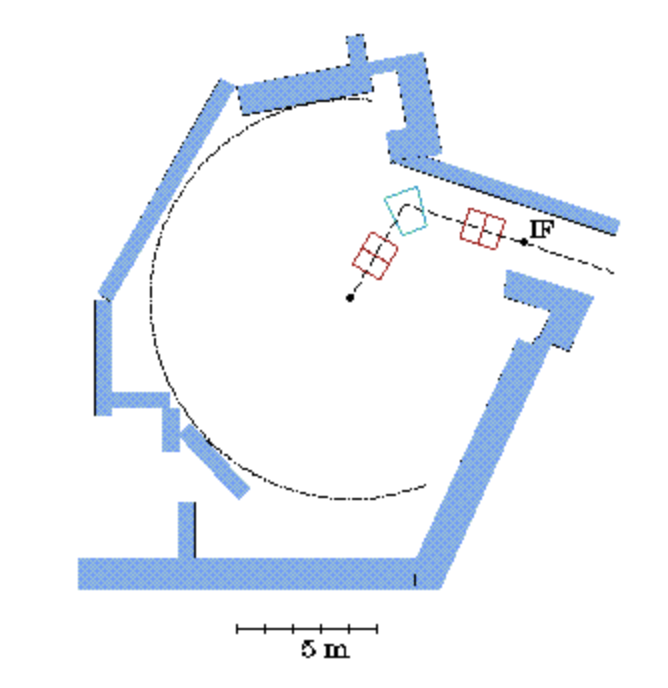
\includegraphics[width=0.35\linewidth]{Experimental area.png}
    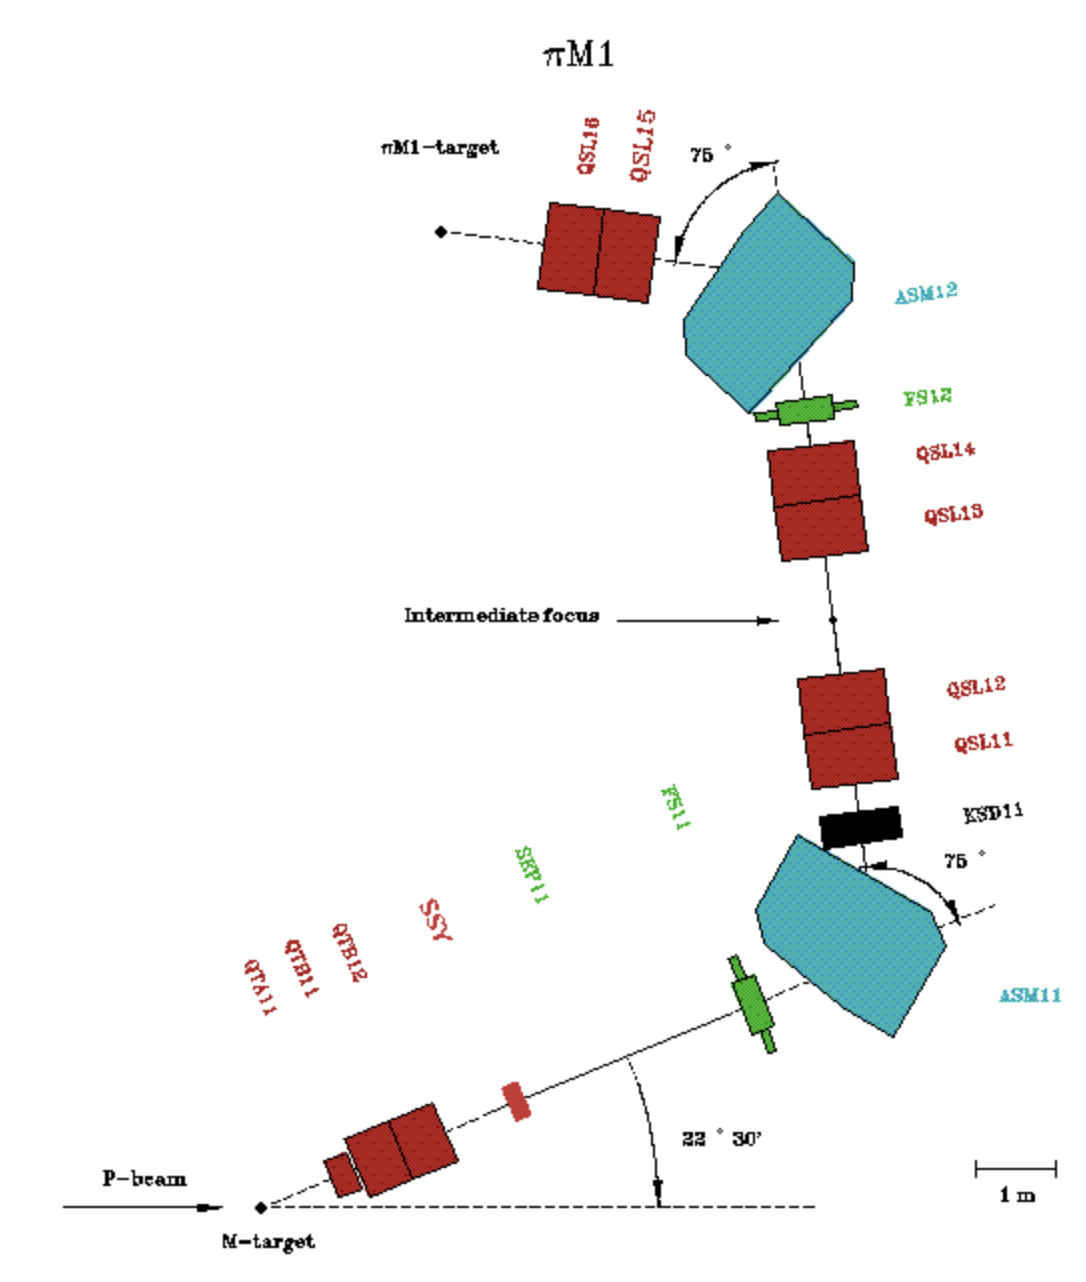
\includegraphics[width=0.45\linewidth]{PiM1.png}
    \caption{Schematic of the $\pi$M1 beamline at PSI. On the left: experimental area where the detector setup was installed. On the right: Beam transport system including dipole and quadrupole magnets as well as collimators used to select and focus the secondary beam. Adapted from~\cite{PSI PiM1}.}
    \label{piM1}
\end{figure}


The present experiment was performed at the High Intensity Proton Accelerator (HIPA) facility at PSI, in the $\pi$M1 beamline area (see Fig.\ref{piM1}). This beamline provides a high-intensity pion beam with selectable momentum in the range of 100–500 MeV/c. In addition to pions, the beam contains muons and positrons/electrons originating from pion decays and electromagnetic interactions, though at significantly lower intensities.



\subsection{Detector system} 
To carry out the experiment, plastic scintillators coupled to photomultiplier tubes (PMTs) were employed as the main detection devices. These detectors were used to register the passage of charged particles from the beam as well as the decay products emerging from the target. The scintillators provided precise timing information, while the use of additional veto detectors allowed background suppression and event selection.
\subsubsection{Functioning of scintillators and PMTs}
The detection principle of a scintillator coupled to a PMT is based on the conversion of the energy deposited by a charged particle into a measurable electrical pulse. When a particle traverses the scintillator material (plastic in this case), its molecules are excited; as they return to their ground state, they emit photons in the visible range. These photons are guided through the scintillator to the photocathode of the PMT, where they are converted into electrons via the photoelectric effect. Inside the PMT, the electrons are accelerated and multiplied through a cascade of dynodes held at successively higher voltages, resulting in an amplification by several orders of magnitude. Since the trajectories of the photoelectrons inside the PMT are very sensitive to magnetic fields, the tube is surrounded by a layer of magnetic shielding material to prevent deflection. The amplified signal appears as a fast electrical pulse at the PMT anode, which can then be read out using an oscilloscope or appropriate timing electronics.
A schematic overview of the detector geometry is shown in Fig.\ref{Pulse}.
\begin{figure}[h]
    \centering
    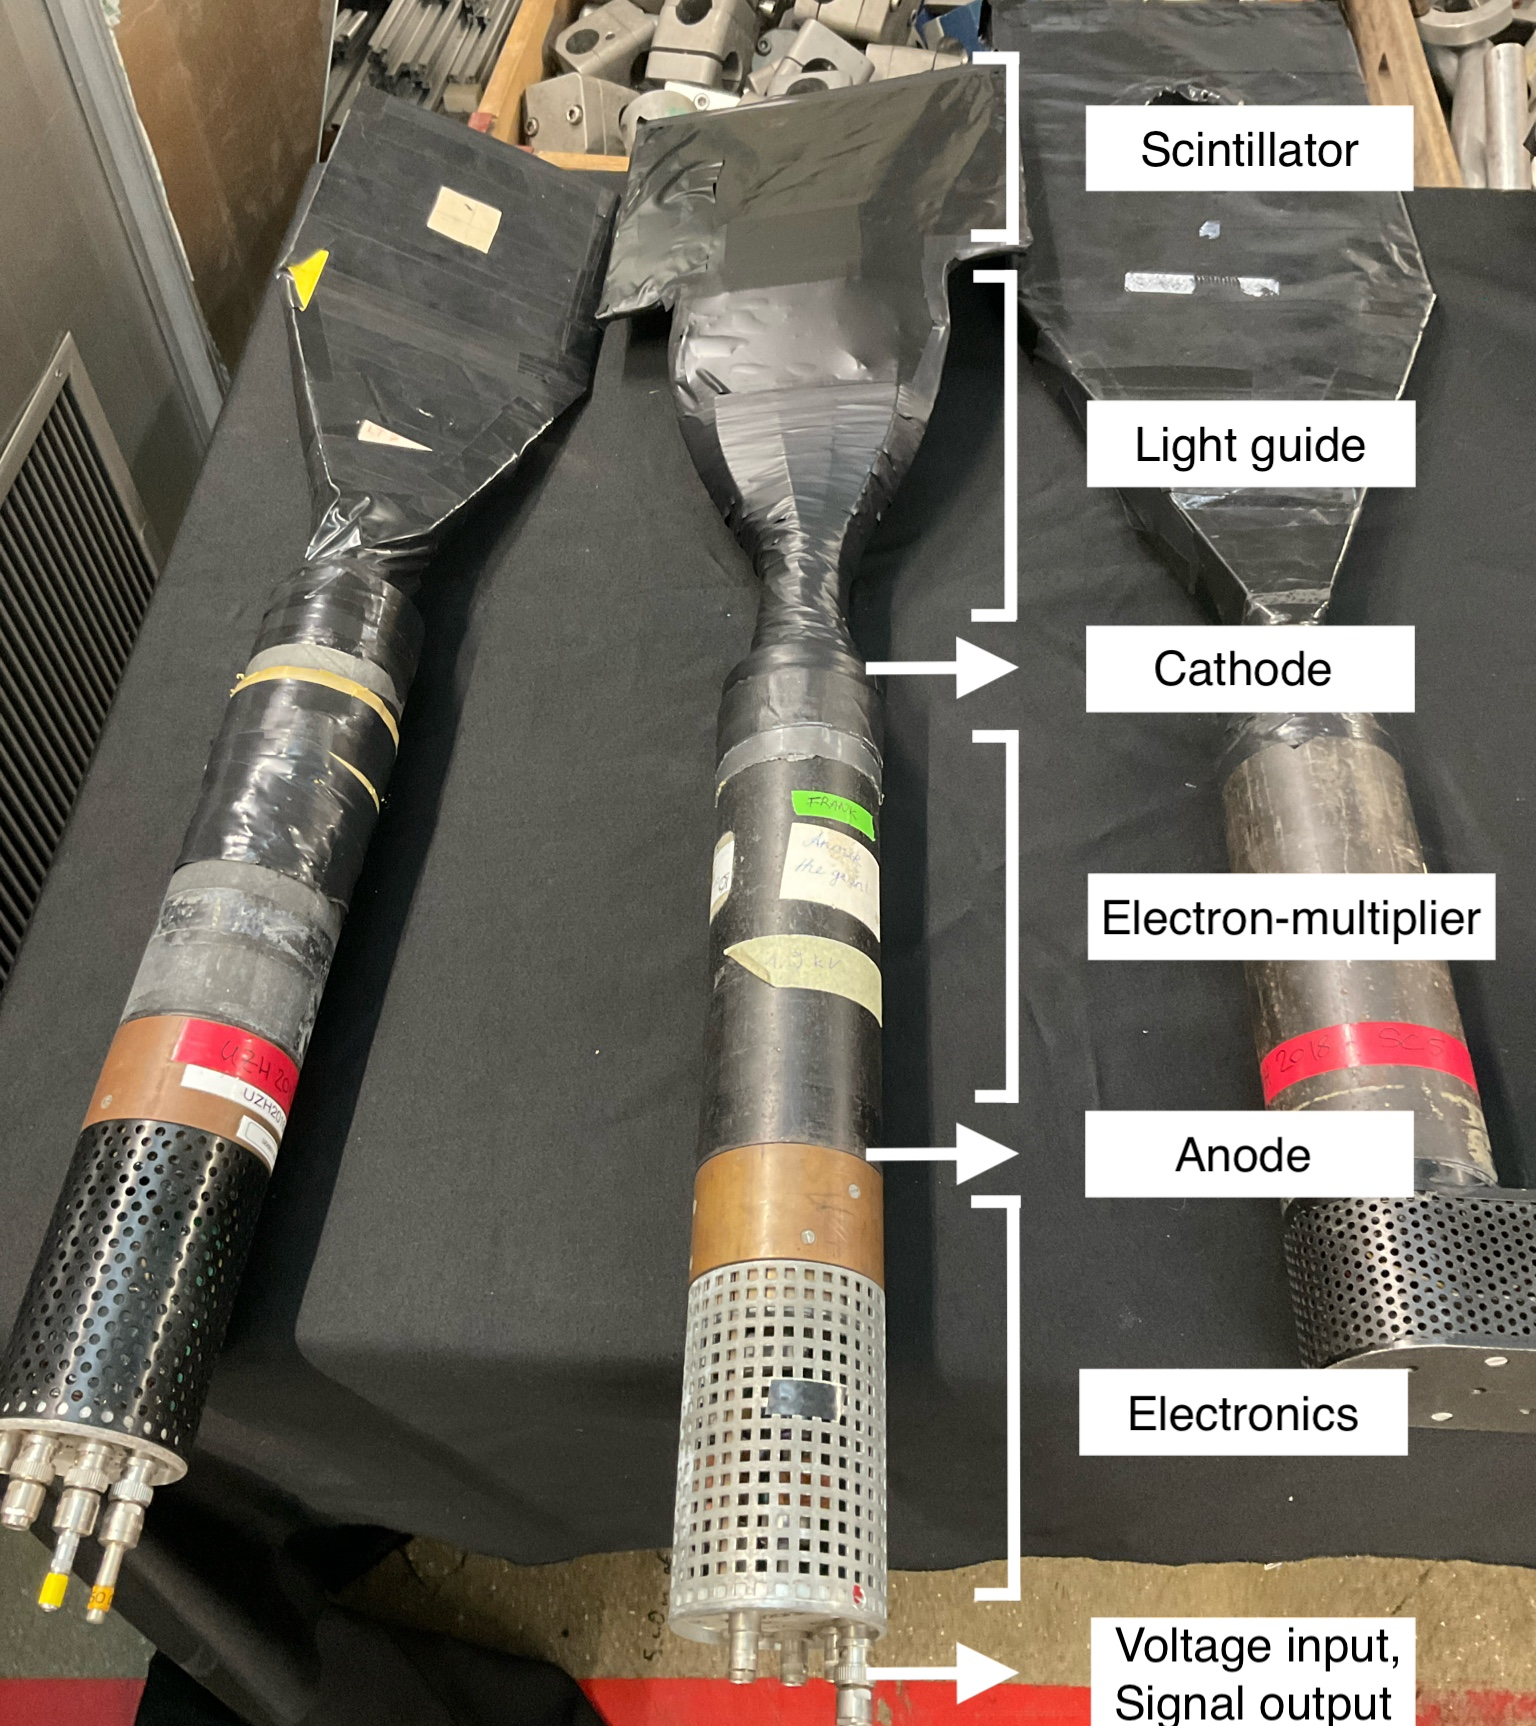
\includegraphics[width=0.45\linewidth]{Detector.jpeg}
    \caption{Picture of the main components of the detector used in the experiment. On top the scintillators attached at the bottom the PMTs with a hole for the signal emission.}
    \label{piM1}
\end{figure}

PMTs also generate spurious signals due to thermal excitation of the photocathode or photons originating from external sources. Such noise pulses can be mistakenly counted as valid events. To reduce this effect, some detectors were implemented in pairs, requiring coincident signals in both scintillators. This coincidence condition strongly suppresses random noise while preserving true particle events.

\subsubsection{Oscilloscope testing}

To verify the proper functioning of the scintillators and oscilloscopes, a $\beta$-emitting source was used. After applying the appropriate high voltage to the PMTs and connecting their outputs to an oscilloscope, the detection capability was tested using a small piece of $^{90}$Sr placed close to the scintillator. When more than one output signal was used, a standard 50 $\Omega$ termination was connected directly to the secondary output of the scintillator module to avoid noise due to signal reflections.
The emitted $\beta$-particles produced scintillation light, which was converted into electrical pulses by the PMT. On the oscilloscope, these signals appeared as sharp negative peaks (see Fig. \ref{Pulse}). A clear difference between the measurements with and without the source confirmed the correct operation of the detectors. 

\begin{figure}[h]
    \centering
    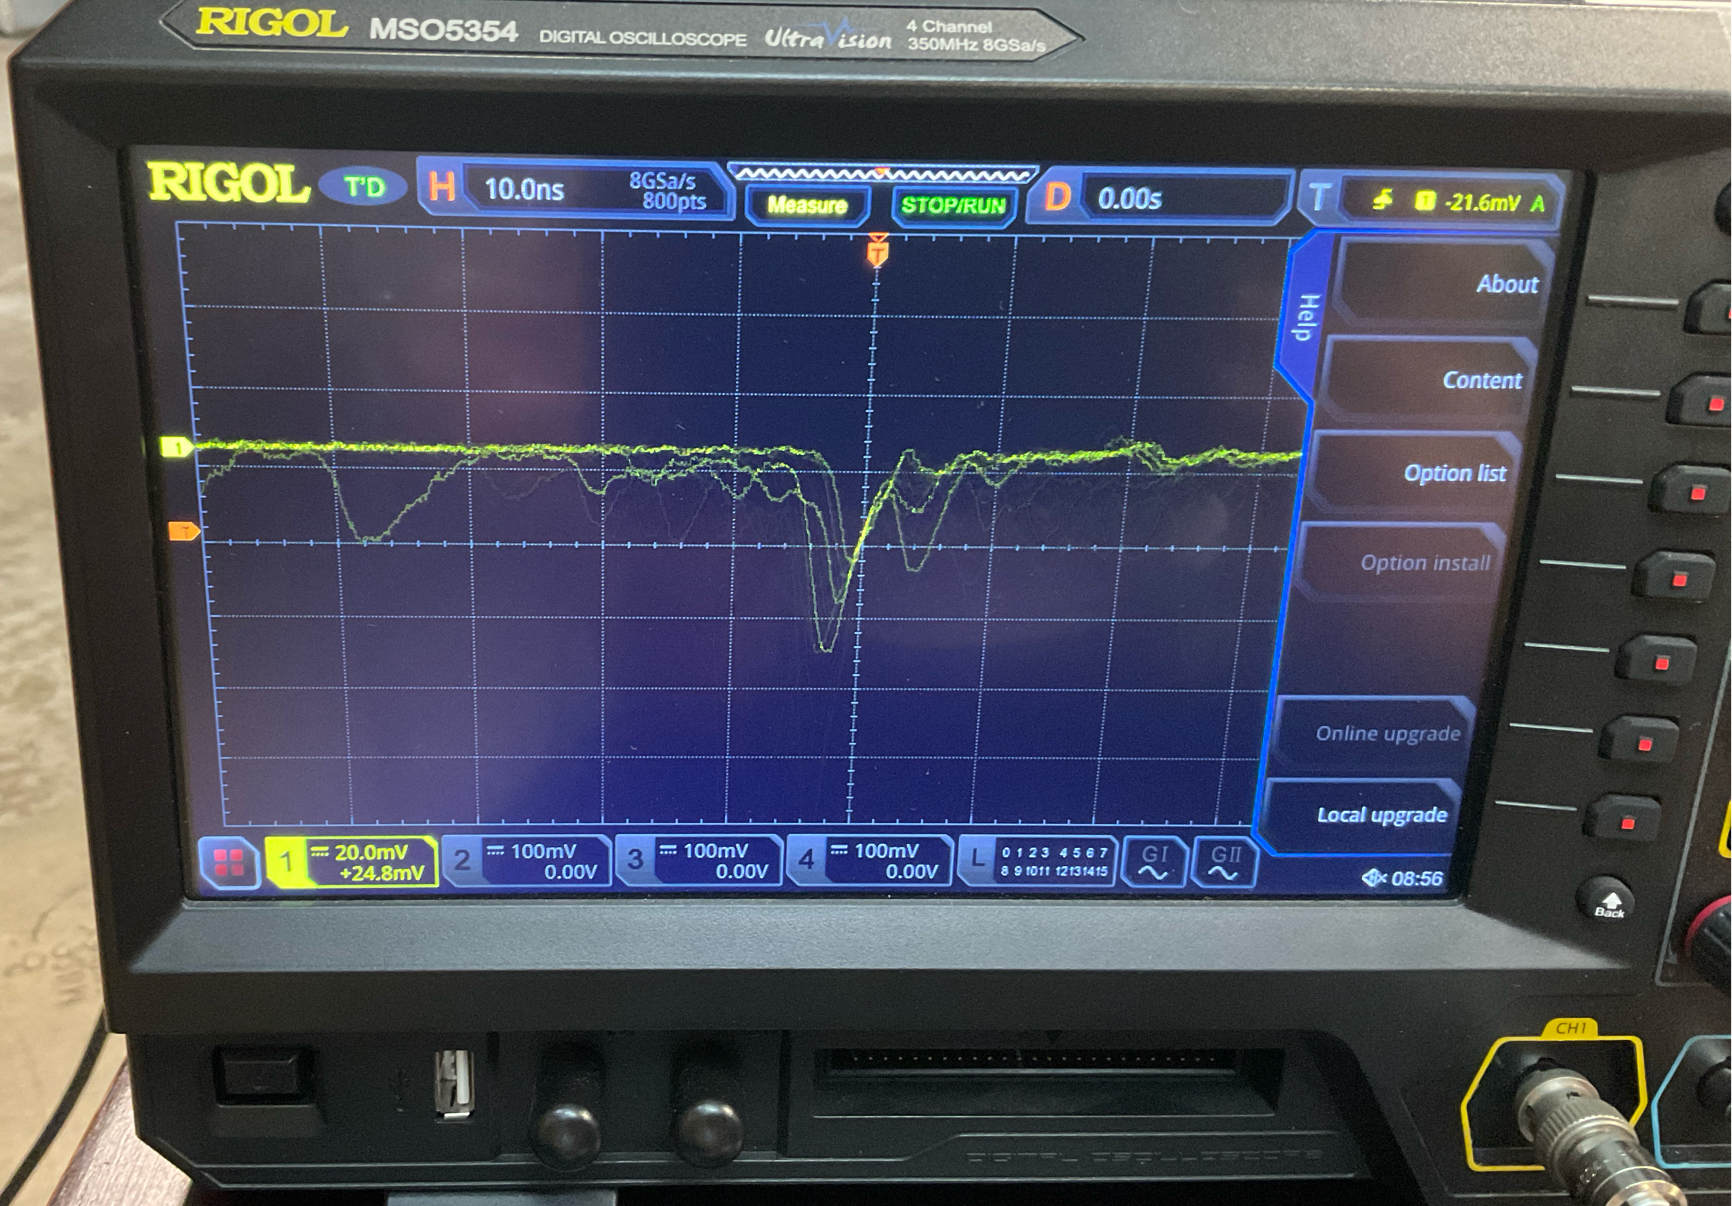
\includegraphics[width=0.45\linewidth]{Noise.jpeg}
    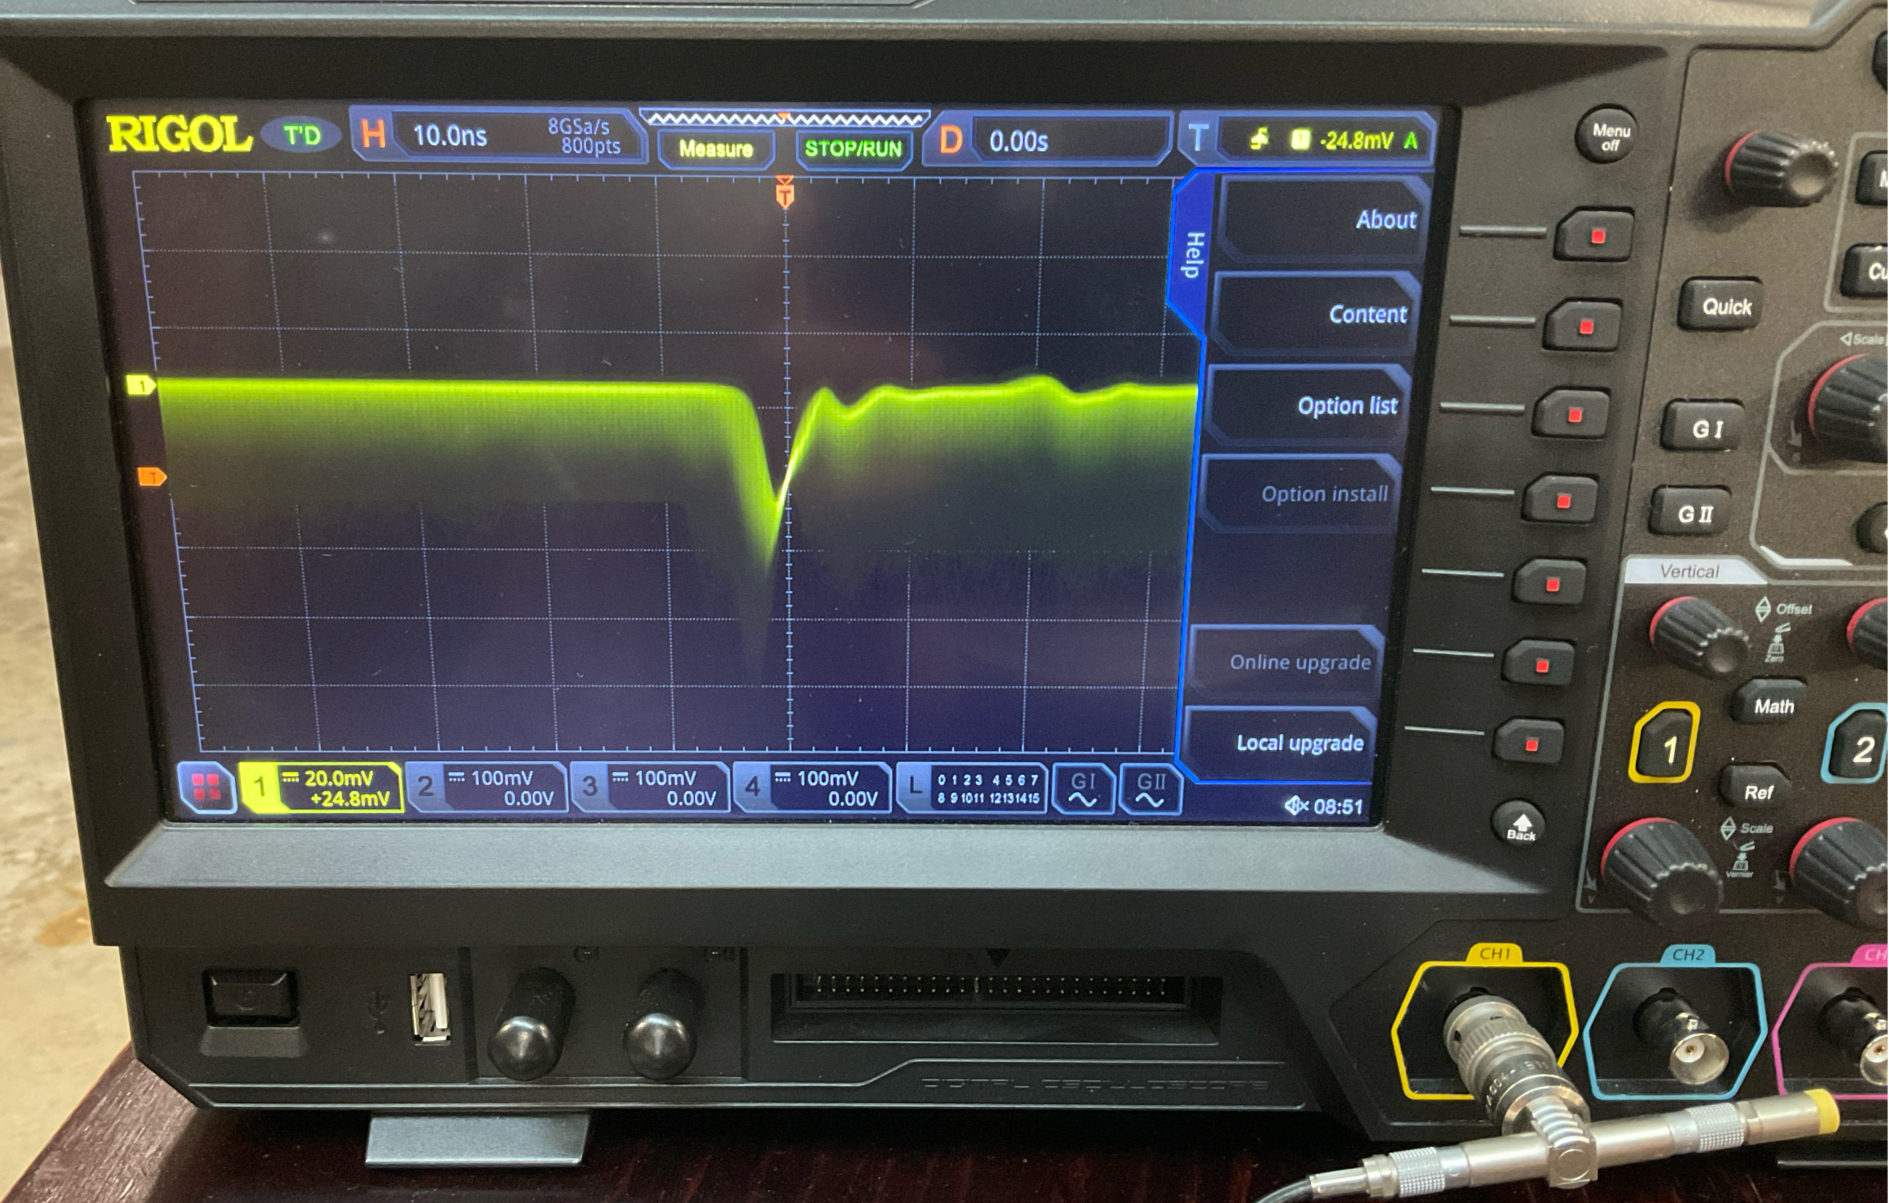
\includegraphics[width=0.45\linewidth]{Sr90.jpeg}
    \caption{Oscilloscope traces recorded during detector testing. Left: spurious noise signals without source. Right: distinct negative pulse produced by $\beta$-particles from the $^{90}$Sr source.}
    \label{Pulse}
\end{figure}

\subsubsection{Experiment configuration}
\label{config}
For this experiment, seven plastic scintillators of different shapes and operating voltages were used (see Table \ref{tab: scint}). The detectors were mounted on a support structure made  out of metal rods and nuts and positioned along the beamline directly downstream of the last quadrupole magnet. Figure \ref{setup} shows both a photograph of the final setup and a schematic sketch of the detector arrangement.
\begin{table}[h!]
    \centering
    \begin{tabular}{|c|c|c|}
    \hline
       Scintillator & Length x Width [cm] & Thickness [cm] & Voltage [kV]\\ \hline
       1 & 18 x 18 & 0.3 & 2.1 \\ \hline
       2 & 10 x 10& 0.6 & 2.1 \\ \hline
       3 & 4 x 4& 0.7 & 2.1 \\ \hline
       4 & 15 x 13 &1.0 & 2.2 \\ \hline
       5 & 34 x 28& 2.1 & 2.0 \\ \hline
       6 & 10 x10 &1.0 & 2.0 \\ \hline
       7 & 10 x10&0.4 & 2.0 \\ \hline  
    \end{tabular}
    \caption{Overview of the seven scintillators and their respective thickness and applied voltage.}

    \label{tab: scint}
\end{table}

When determining the distances between the individual detector components, two main factors were taken into account. First, the detectors could not be placed too close to each other, in order to minimize noise signals originating from scattered particles in the upstream detector. On the other hand, excessively large separations were also avoided, since particles traversing long distances in air would lose energy according to the Bethe–Bloch formula. As a compromise between these two effects, a detector spacing of 15-20 cm was chosen.

\begin{figure}[h]
    \centering
    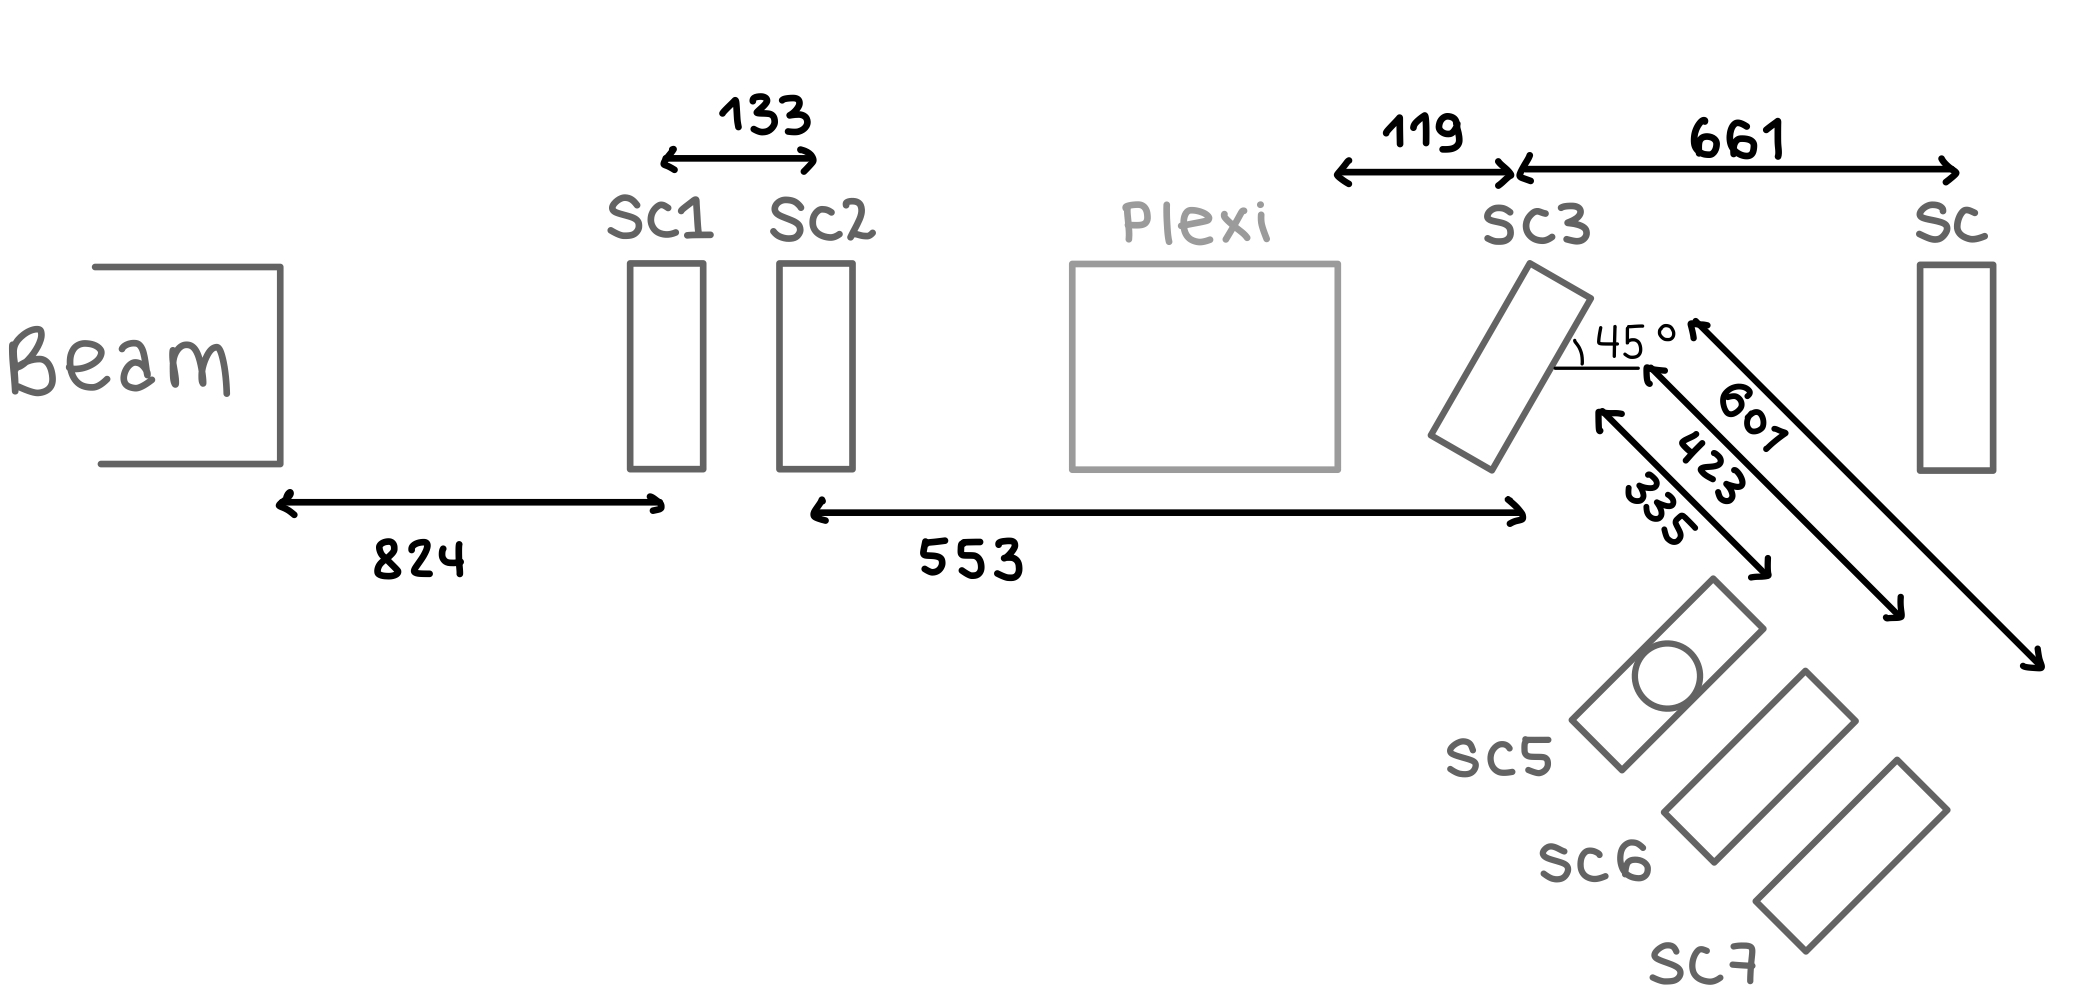
\includegraphics[width=0.49\linewidth]{Set up 1.jpeg}
    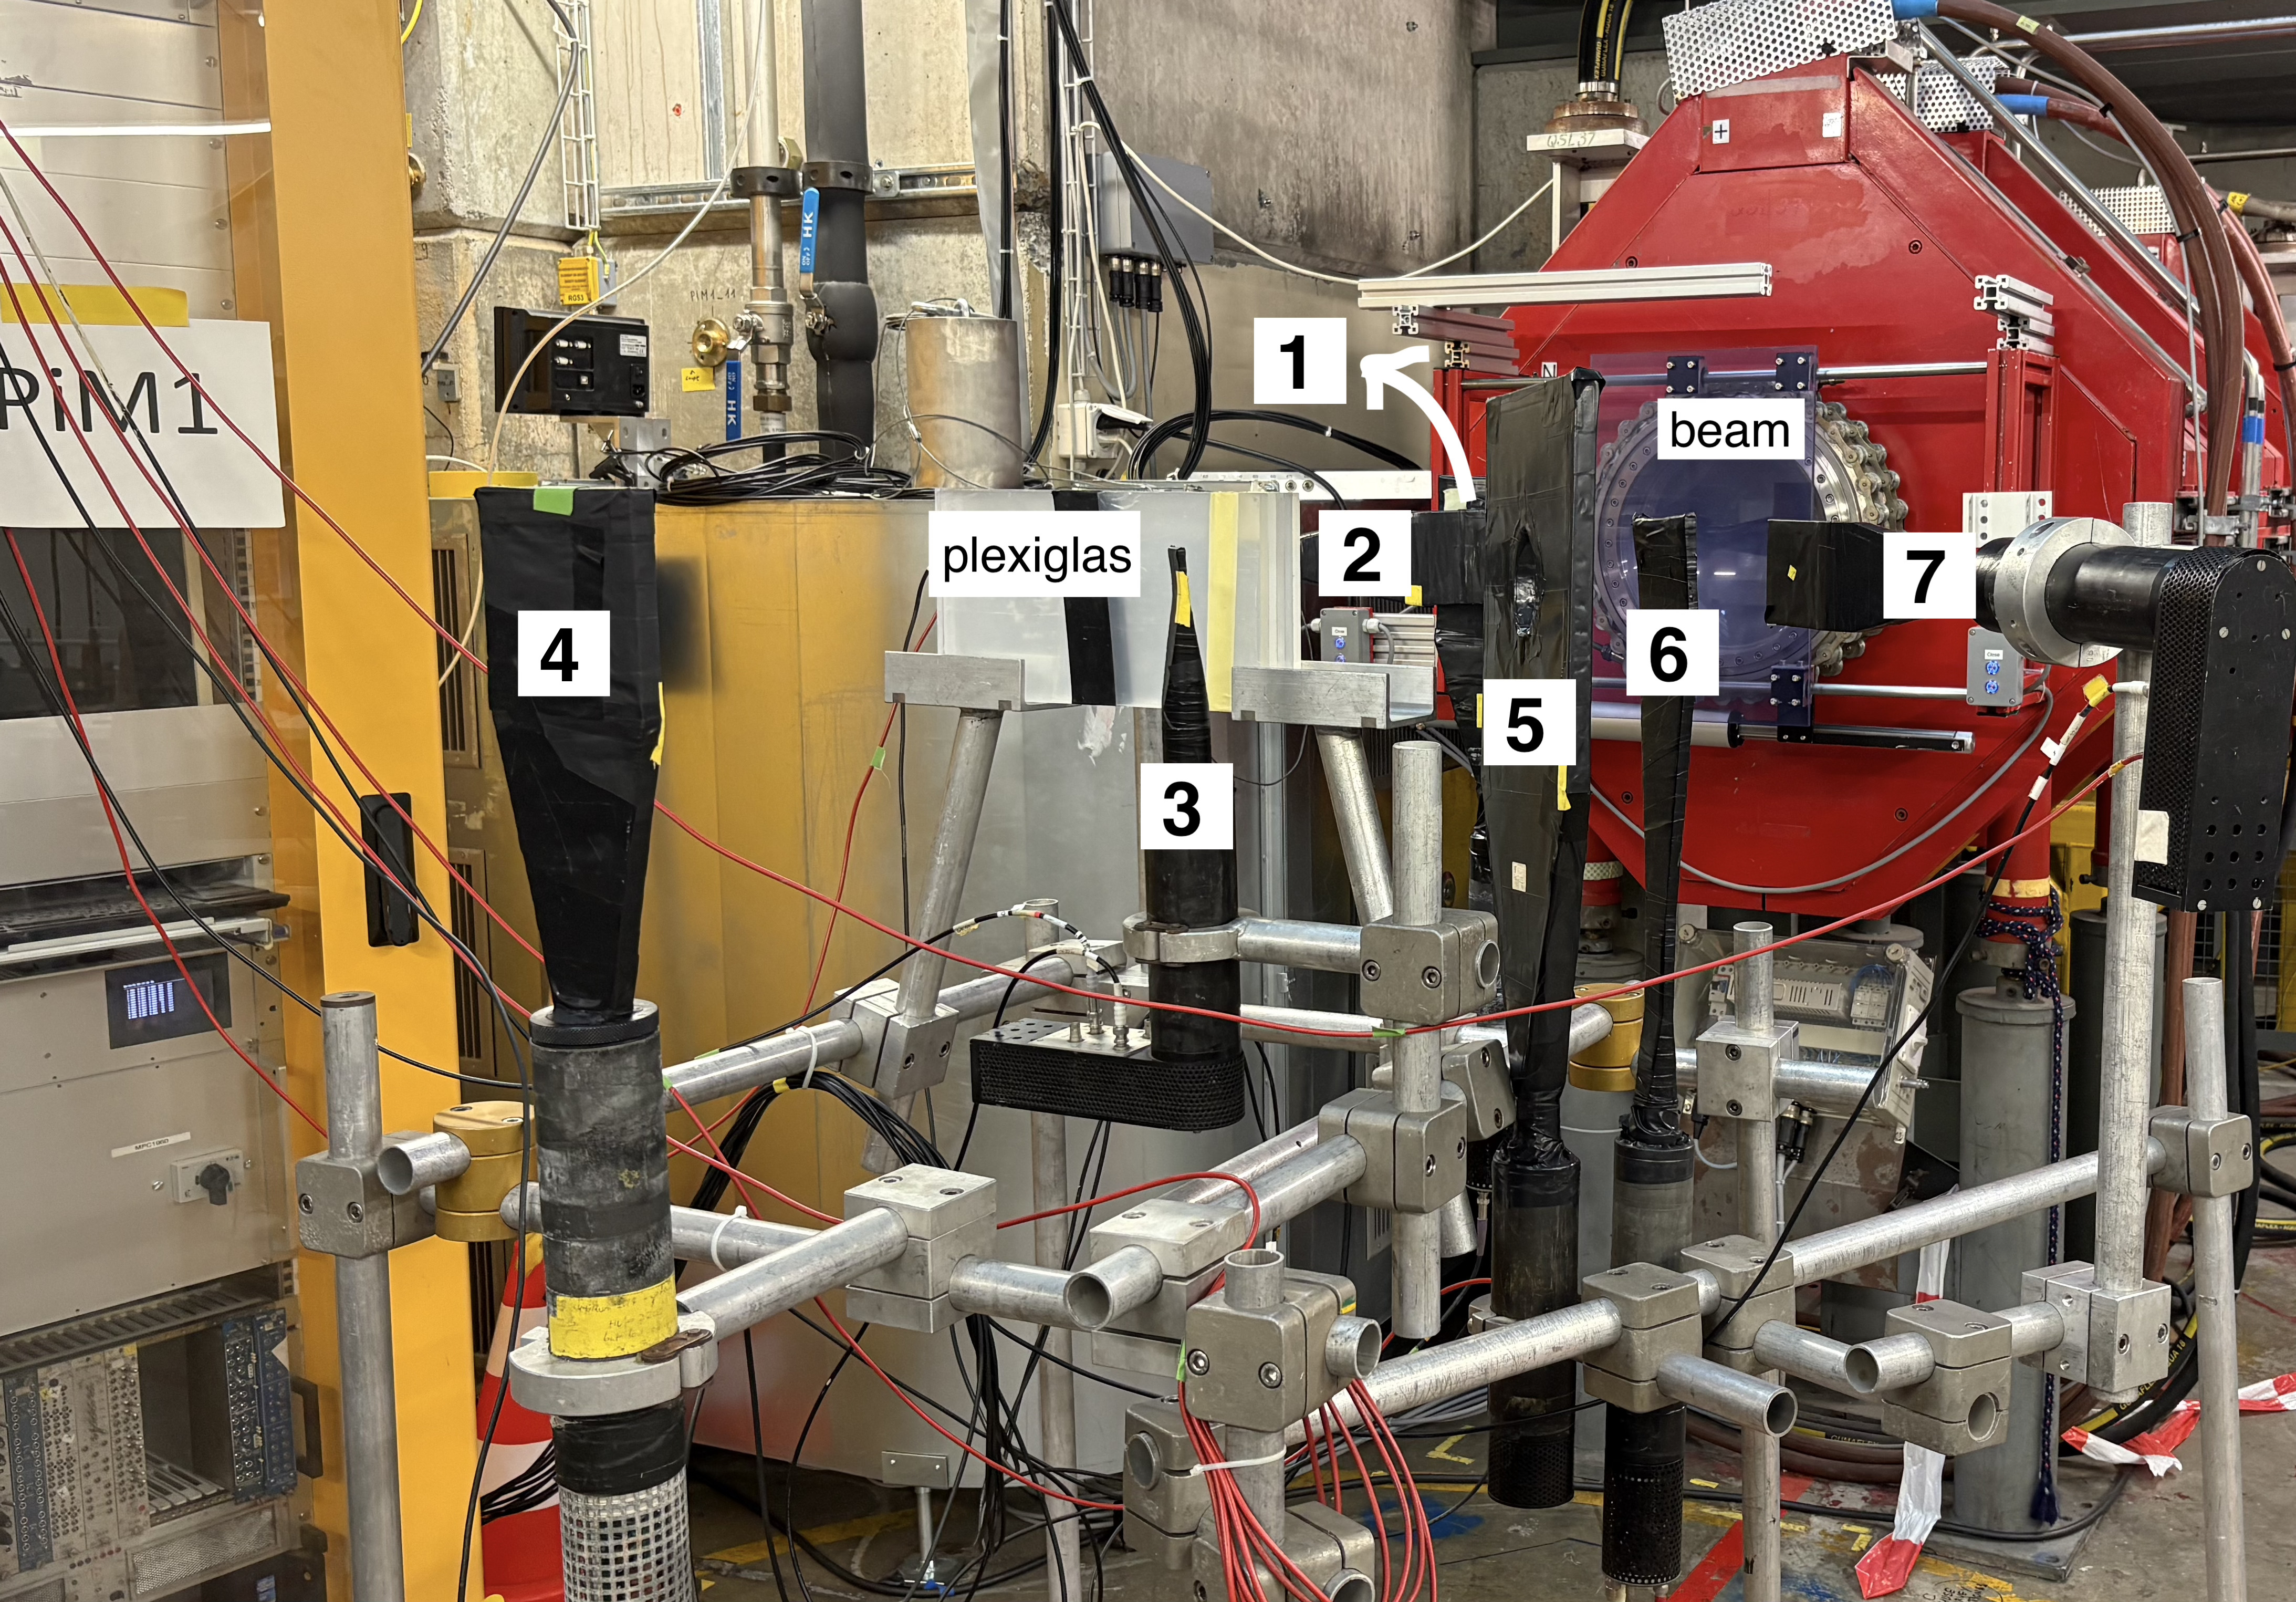
\includegraphics[width=0.45\linewidth]{Set up 2.jpg}
    \caption{Photograph of the experimental setup (right) and schematic sketch indicating the relative positions and distances [mm] between the scintillators (left). Note that scintillator 4 was repositioned during the setup, but the updated distance wasn't recorded.}
    \label{setup}
\end{figure}

The beam first passed through two small scintillators (S1 and S2), which  ensured that only particles coming from the beam, and not from the surrounding area, were considered for the experiment.

At the target position, a thin scintillator (S3) was installed to stop incoming pions and muons and to define the start time of the lifetime measurement. Its thickness was chosen such that positrons did not stop in it. Since the pions carried too much energy to be fully stopped in such a thin detector, an 8 cm plastic buffer was placed upstream to slow them down. The target was tilted by 45° with respect to the beam axis: this orientation provided a larger effective surface to the beam while simultaneously reducing the escape path length for positrons, thereby increasing the probability that they reached the stop detector instead of scattering inside the material.

A fourth scintillator (S4) was placed in the beamline directly downstream of the target and used as a veto counter. In this configuration, any particle that did not stop in the target (such as through-going muons or positrons from the beam) produced a signal in S4, which in anti-coincidence with the main detectors suppressed such events from the dataset.

The remaining three detectors (S5–S7) were placed approximately 135° off-axis. This geometry reduced the rate of background from forward-scattered particles, which are more frequent at smaller angles. Scintillator S5, which contained a central hole, acted as a veto for the stop signal: only positrons from the target passed through the hole without producing a signal, while scattered particles striking S5 triggered a veto and suppressed accidental coincidences. Downstream of S5, two further scintillators (S6 and S7) registered the decay positrons, providing the stop signals for the lifetime measurement.

This arrangement allowed a clear definition of the incoming beam and precise measurement of the decay-time spectrum.



\subsection{Electronics and trigger logic}
\label{Electronics and triger logic}
The output signals from each detector were guided to the control room using cables of equal length, in order to avoid additional time delays. 

The readout electronics of the experiment were assembled from NIM (Nuclear Instrumentation Module) units housed in a standard crate in the control room.
NIM defines mechanical and electrical specifications for laboratory electronics, including common DC voltages and standardized connectors.

In our setup, the readout chain followed the sequence:
\[
\text{PMT signals} \rightarrow \text{Amplifiers} \rightarrow \text{Discriminators} \rightarrow
\text{Coincidence + Delay} \rightarrow \text{TAC} \rightarrow \text{ADC} \rightarrow \text{Computer}.
\]

The signals from the scintillators were collected by PMTs, amplified, and converted into logic pulses by discriminators.
Coincidence and veto conditions, together with calibrated delay cables, were then used to form the two essential timing signals:

\begin{itemize}
    \item \textbf{START} signal: $(\text{S1} \land \text{S2} \land \text{S3} \land \lnot \text{S4})$, corresponding to a pion stopping in the target;
    \item \textbf{STOP} signal: $(\text{S6} \land \text{S7} \land \lnot \text{S5})$, corresponding to the detection of the decay positron.
\end{itemize}

The time difference between START and STOP was measured by a time-to-amplitude converter (TAC), digitized by an ADC,
and finally recorded on a computer for histogramming.

The following types of modules were employed in the readout chain:
\begin{itemize}
\item Fast analog amplifiers for boosting PMT signals,
\item Discriminators for generating logic signals once the pulse amplitude exceeds a threshold,
\item Coincidence units for combining logic signals and forming the START and STOP triggers,
\item Delay modules (active and passive), including calibrated passive delay cables (1~ns, 4~ns, 8~ns, etc.), for synchronizing signal arrival times,
\item A time-to-amplitude converter (TAC) for generating an analog voltage proportional to the time difference between START and STOP,
\item An analog-to-digital converter (ADC) for digitizing the TAC output and transferring data to the computer,
\item Counters for monitoring trigger rates,
\item A four-channel oscilloscope for monitoring and aligning analog and logic signals.
\end{itemize}

All signals followed the NIM standard logic, and level adapters were available to convert to TTL where required.
The ADC was connected to a Windows laptop running the acquisition software, which displayed and stored the histograms. Data transfer was performed via USB storage devices.\\

In the following sections, the process of creating the trigger logic and the working principles of the different modules are explained.

\subsubsection{Signal amplifiers and discriminators}

The raw PMT signals were first fed into amplifiers to increase their amplitude and ensure a clean processing in the subsequent stages. 

The PMTs deliver negative-polarity analog signals, with amplitudes proportional to the energy deposited by the particles in the scintillators. For the formation of coincidences, these analog pulses needed to be converted into standard logic signals. This was achieved using discriminators. 

In a standard discriminator, a logic output is produced whenever the input signal exceeds a set threshold. However, since signals can have different amplitudes, the threshold is crossed at slightly different times depending on the pulse height. This results in a systematic timing shift, known as \emph{time walk} (see Fig.\ref{CFD}). 

To suppress this effect, constant fraction discriminators (CFDs) were employed. Unlike standard discriminators, they generate the output when a fixed fraction of the pulse height is reached, making the timing independent of the signal amplitude. 



\begin{figure}[h]
    \centering
    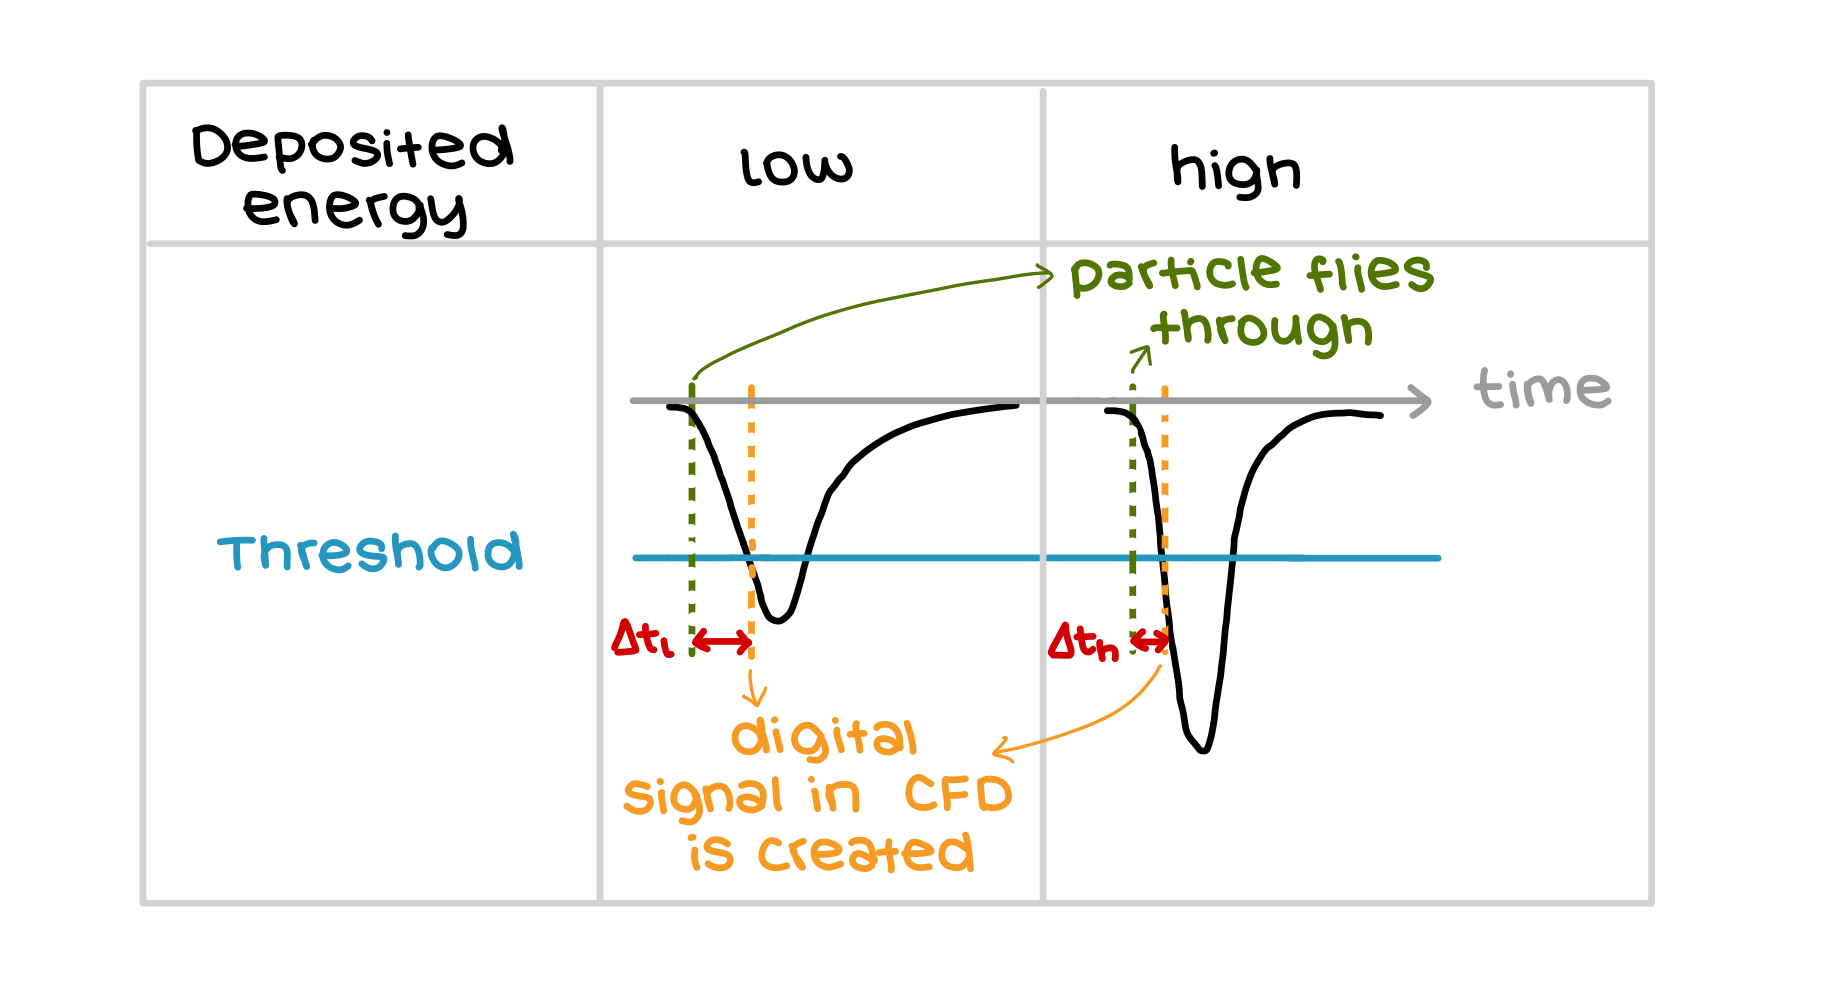
\includegraphics[width=0.48\linewidth]{CFD.jpeg}
    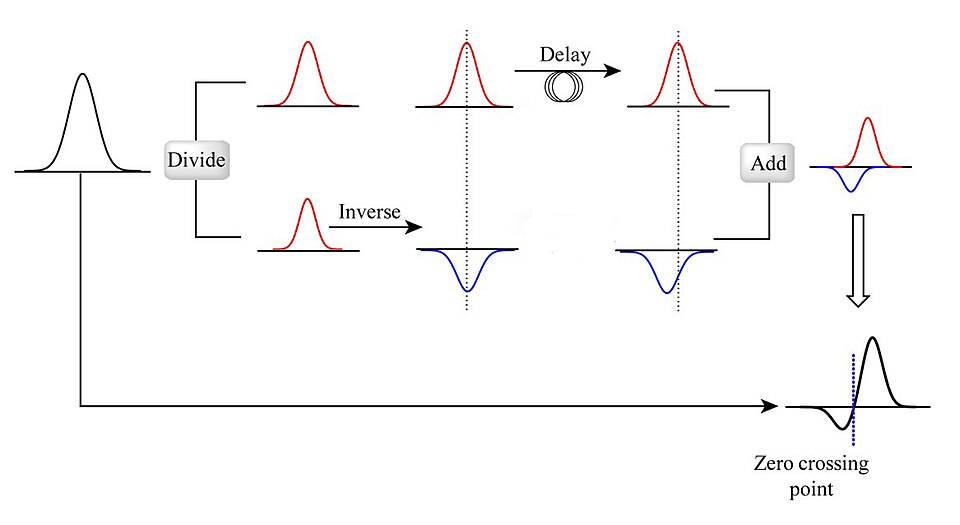
\includegraphics[width=0.48\linewidth]{CFD_Diagram.jpeg}
    \caption{Left: Illustration of the time walk problem in standard discriminators, where the trigger time depends on the input pulse amplitude. Low-energy deposits produce shallower pulses that cross the threshold later, while higher-energy deposits cross earlier, leading to timing shifts. Right: Signal processing steps in a CFD. Adapted from~\cite{CFD}.}
    \label{CFD}
\end{figure}


As illustrated in Fig.\ref{CFD} (right), the CFD splits the input signal into two copies. One copy is attenuated to a fixed fraction of its amplitude and inverted, while the other is delayed by a fixed time interval. When these two signals are summed, they form a bipolar pulse that always crosses the zero line at the same fraction of the original amplitude. The digital output is then generated precisely at this zero-crossing point.  

On the CFD module, two adjustable screws allow fine-tuning of the logic signal width and of the discriminator threshold (see Fig. \ref{Threshold}). The threshold was set high enough to suppress noise, recognizable by high-frequency oscillations in the analog signal and spurious digital outputs with undefined width, while still ensuring that all valid events were retained.


\begin{figure}[h]
    \centering
    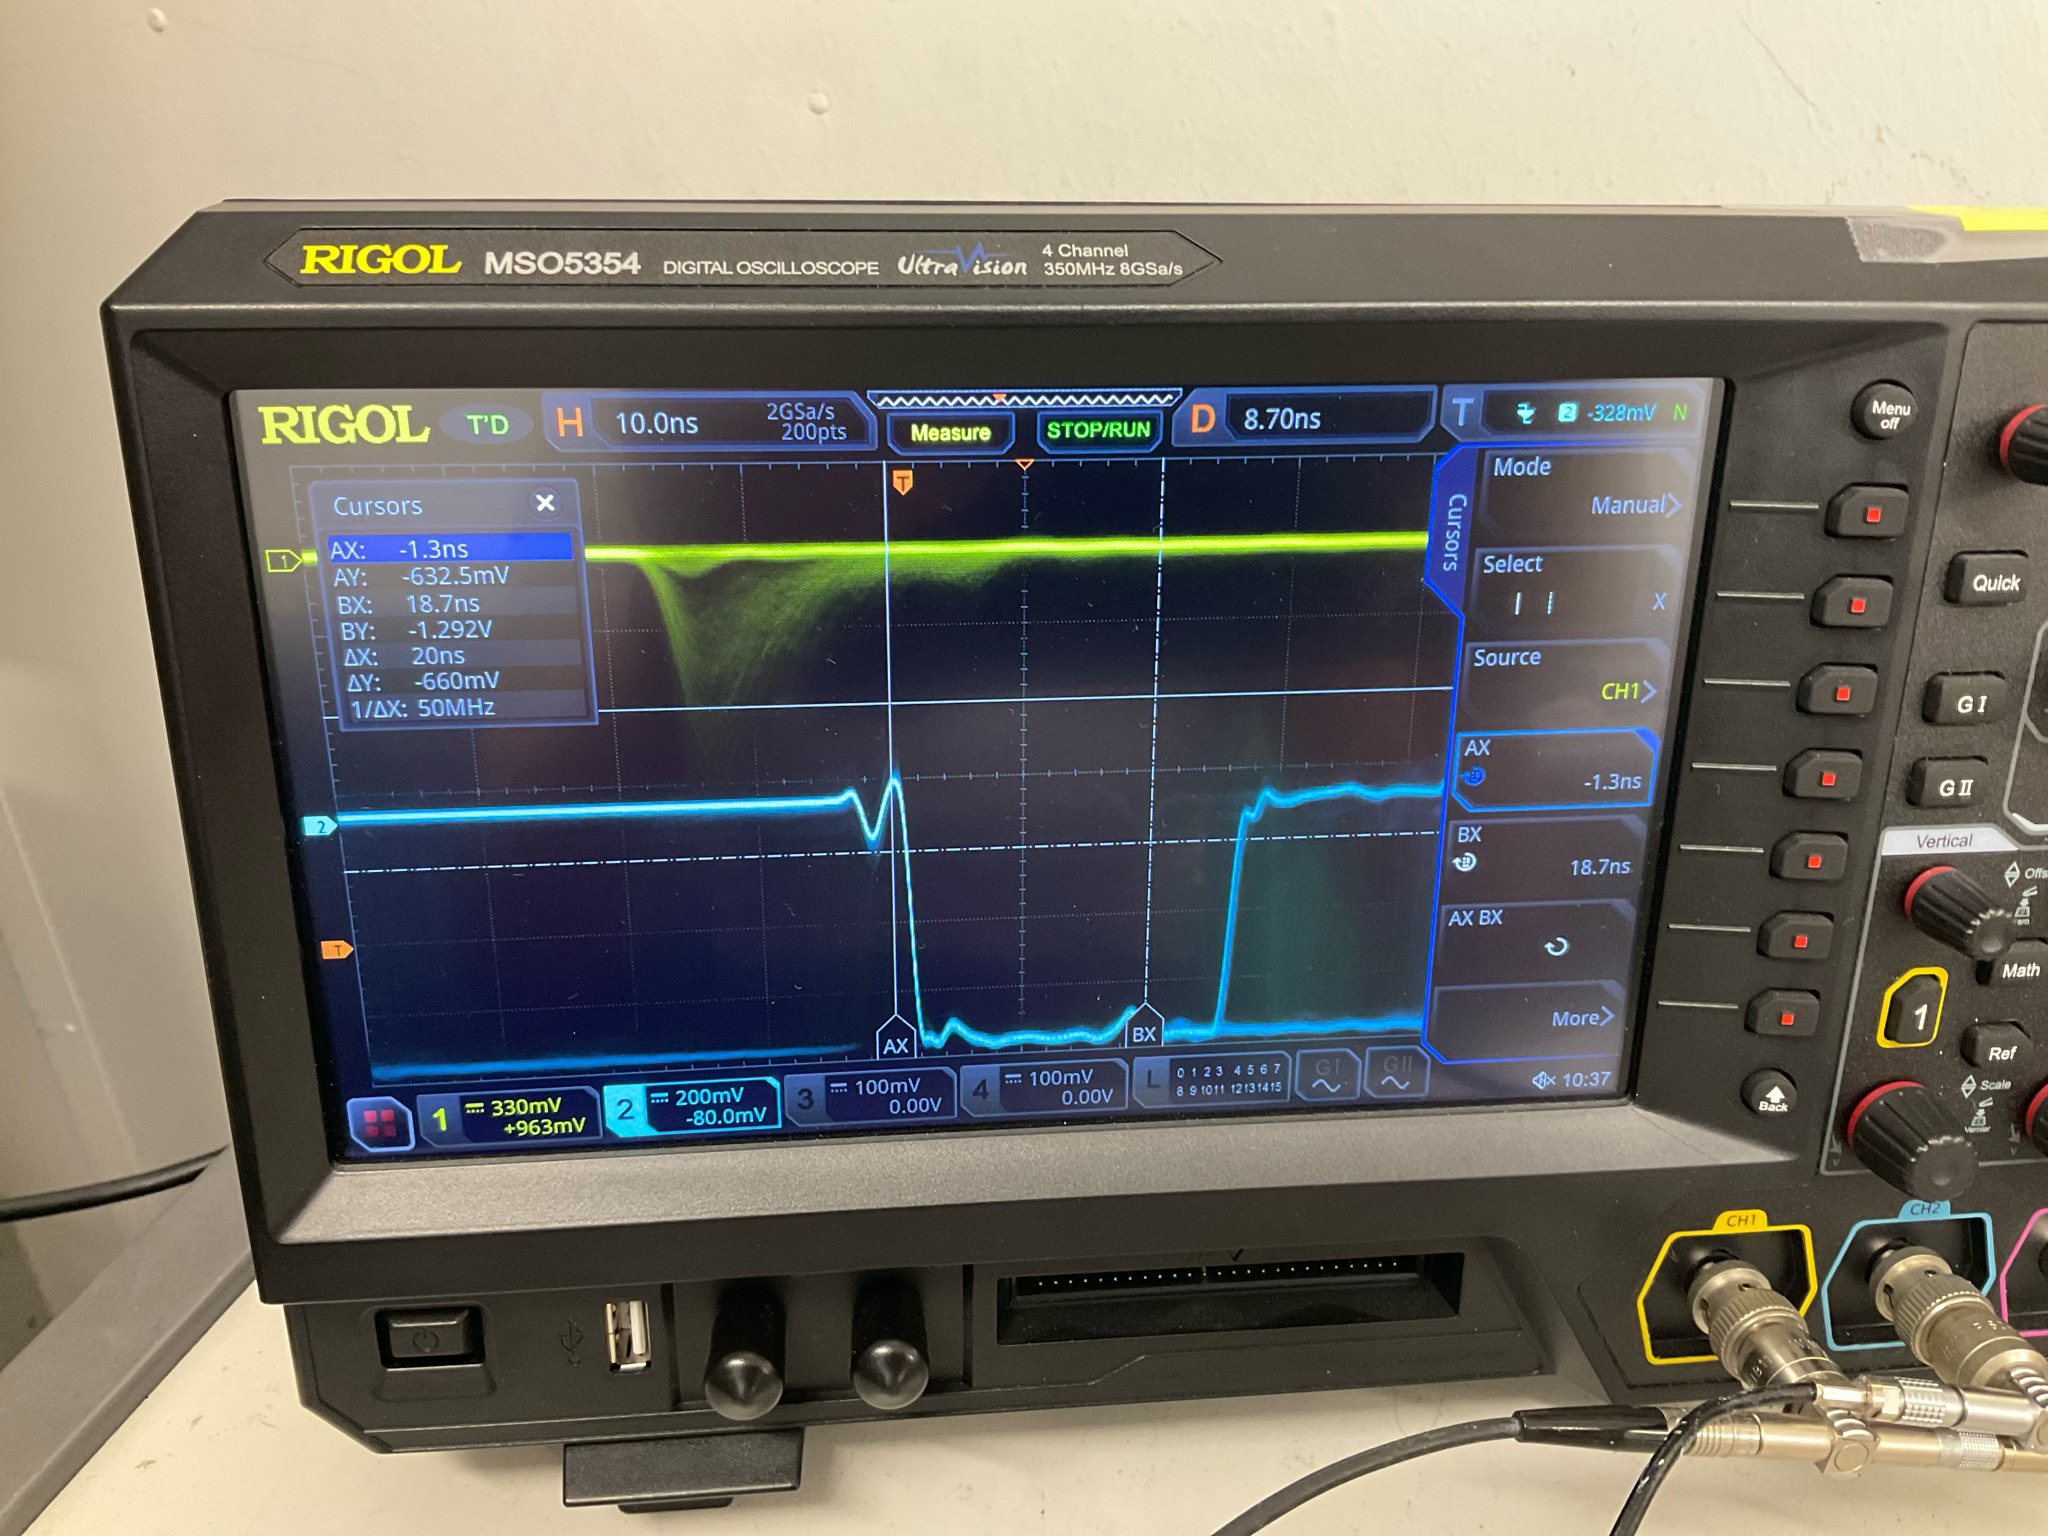
\includegraphics[width=0.48\linewidth]{Low thr.jpg}
    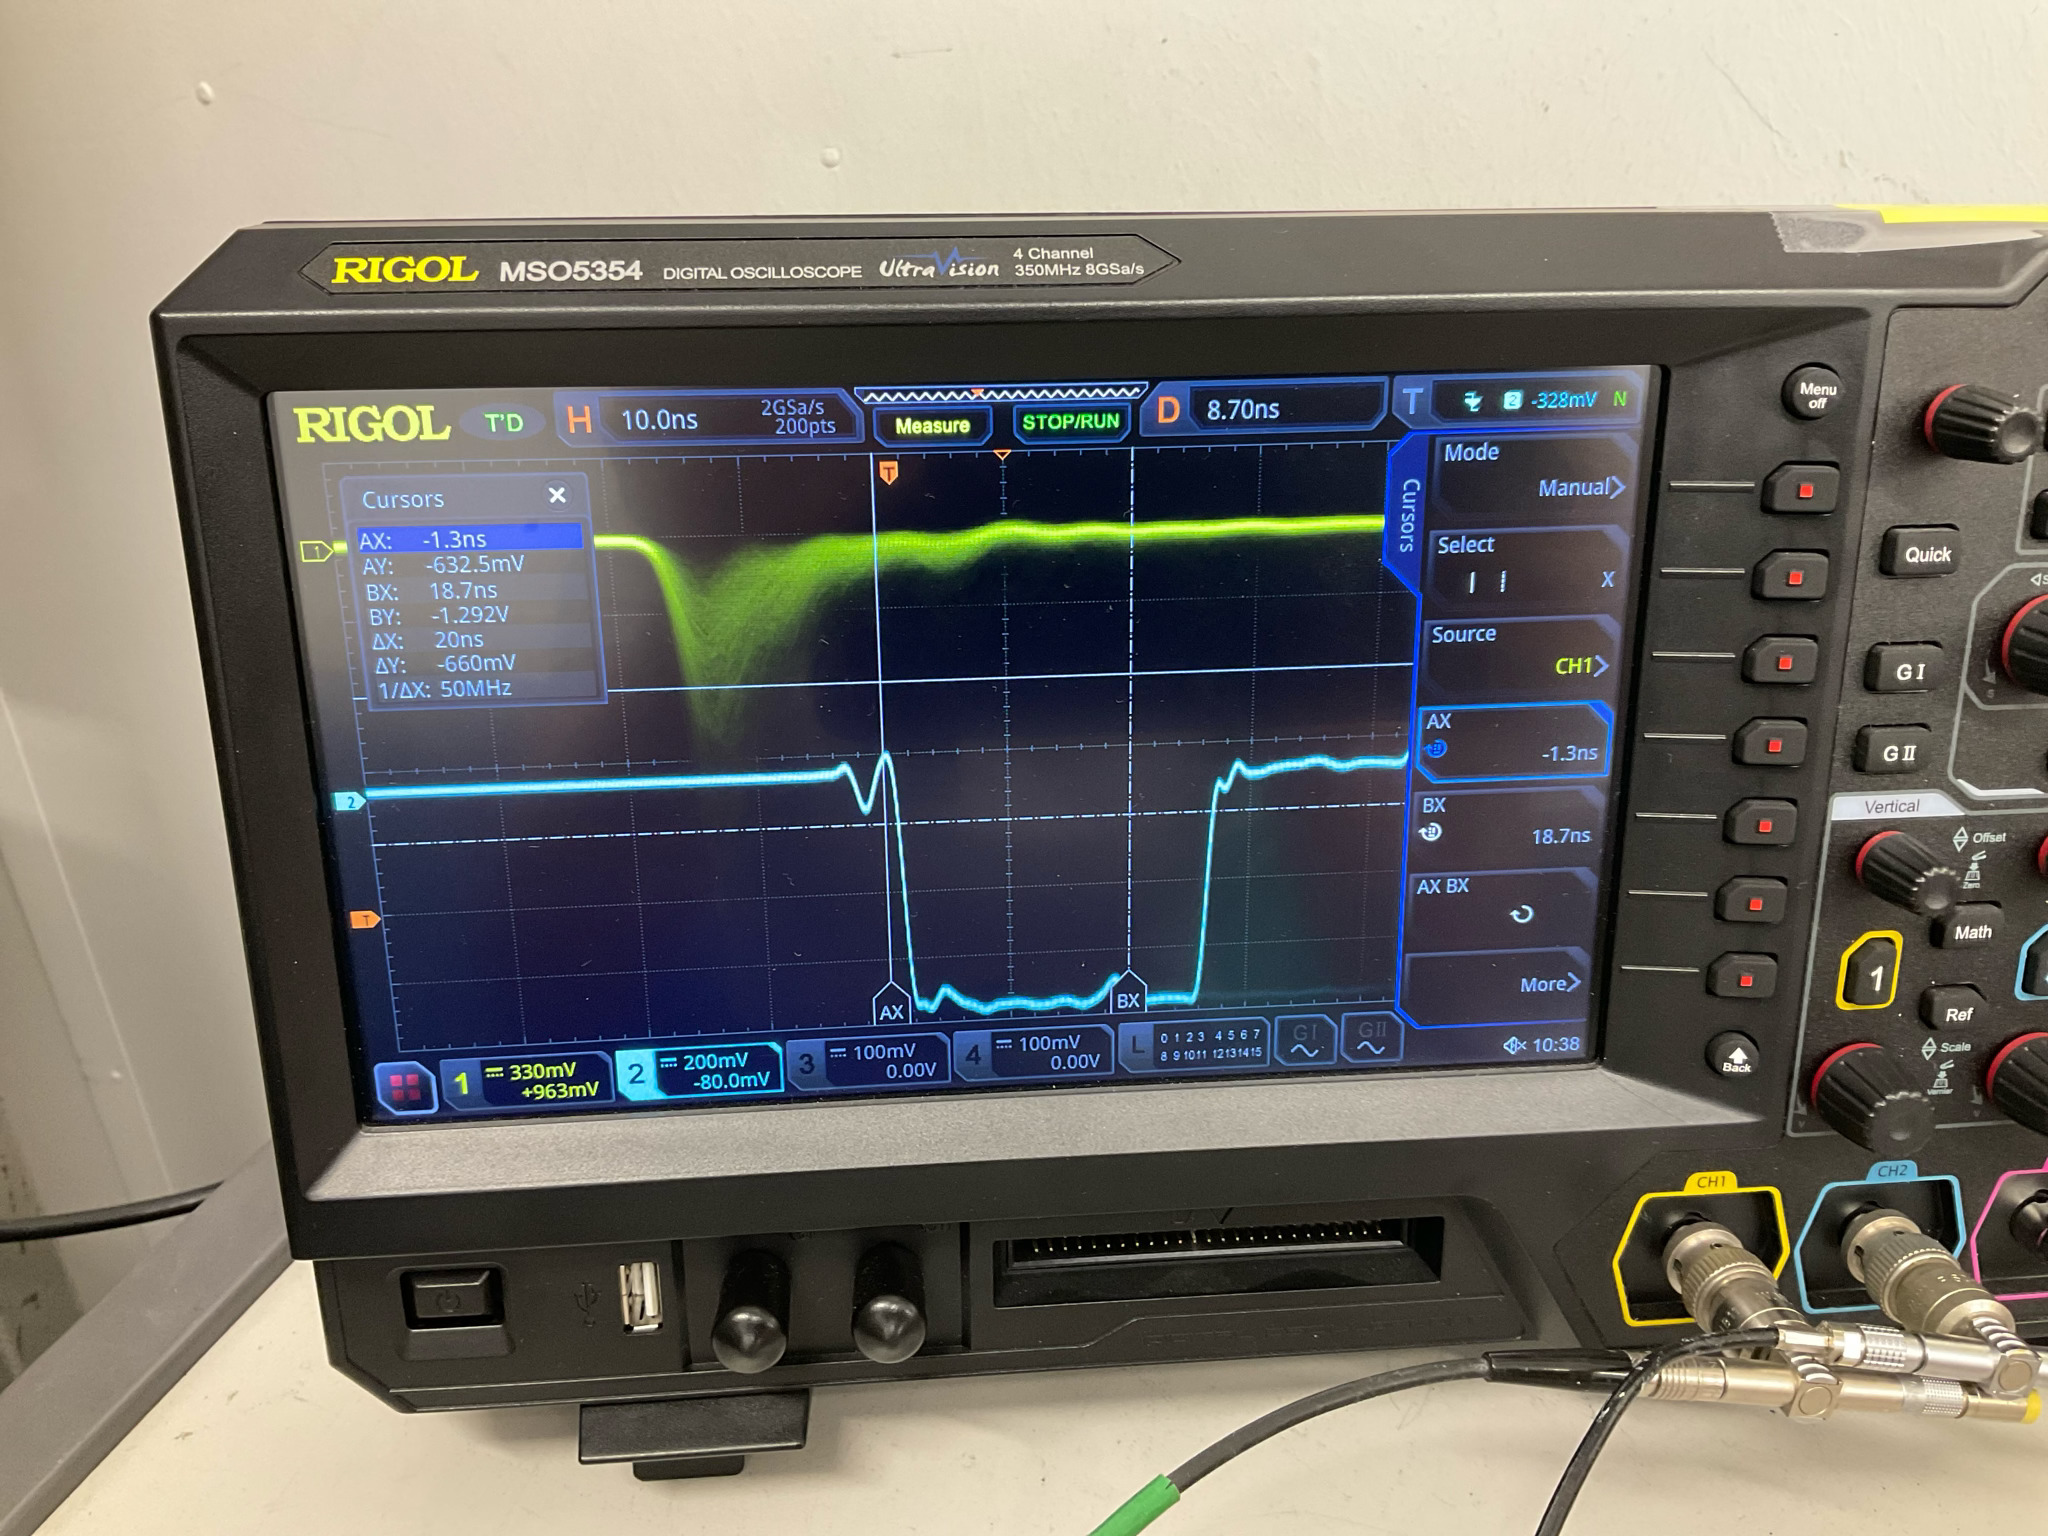
\includegraphics[width=0.48\linewidth]{High thr.jpg}
    \caption{Resulting signals for different discriminator thresholds: low threshold (left) versus higher threshold (right), where the noise is suppressed more effectively.}
    \label{Threshold}
\end{figure}

\subsubsection{Coincidences and START signal}

To perform the logical “AND” operation between two signals, coincidence modules were employed. These modules produce an output signal only when both input signals are present simultaneously. The output is generated at the time corresponding to the later of the two input signals. Therefore, it is crucial to align the relative timing of the inputs, which can be adjusted using delay modules or cables of defined length.  

As described in Section \ref{config}, the START signal for the lifetime measurement was defined as the coincidence of S1, S2, and S3, in anti-coincidence with S4:

\begin{equation*}
    \text{START:} \quad \text{S1} \: \land \: \text{S2}\: \land \: \text{S3} \: \land \: \lnot \text{S4}.
\end{equation*}
    
First, the coincidence of S1 and S2 was formed. This output was then combined in coincidence with S3 (see Fig. \ref{S3}). Since the START signal needed to correspond to the moment when the particle stopped in the target, a 16 ns delay was introduced on the S3 signal using a delay cable, ensuring that the START pulse was generated once the particle passed S3.

\begin{figure}[h]
    \centering
    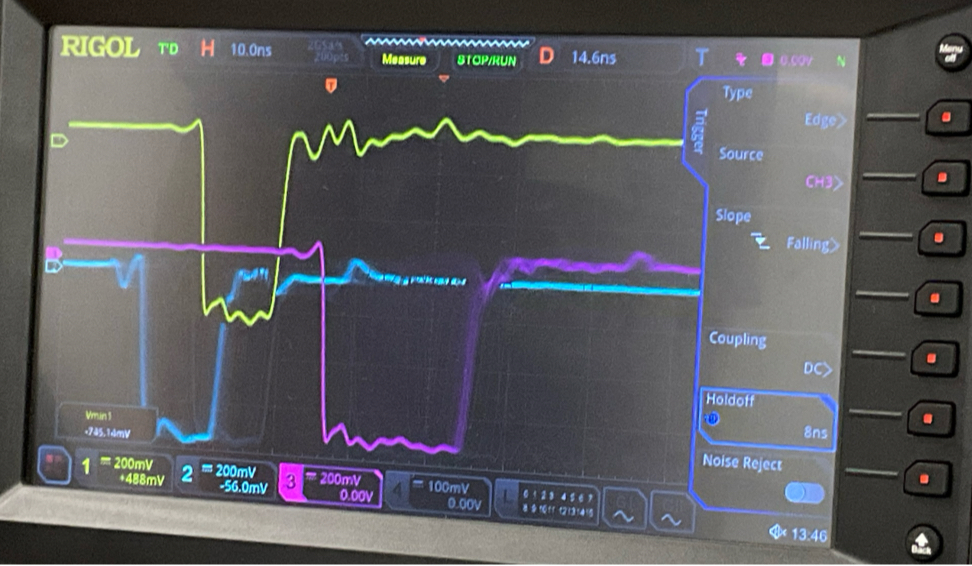
\includegraphics[width=0.48\linewidth]{123.jpeg}
    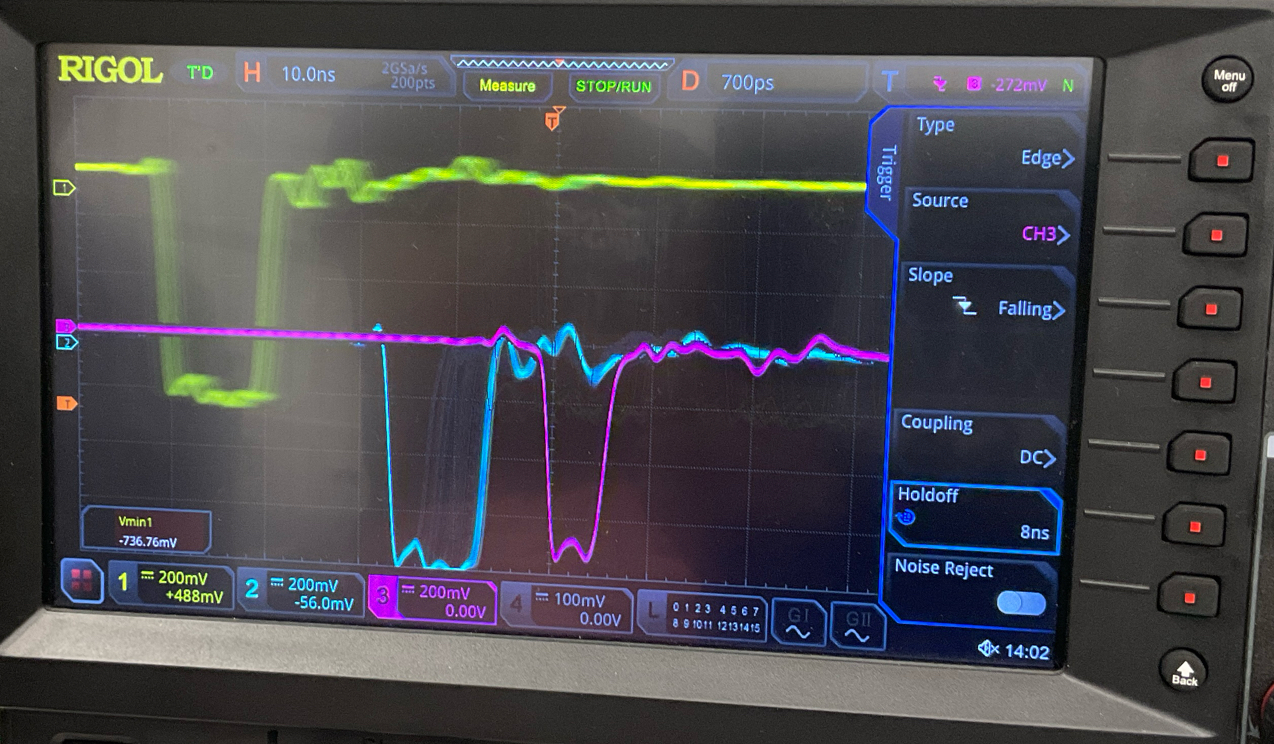
\includegraphics[width=0.48\linewidth]{123 delayed.jpeg}
    \caption{Coincidence of S1, S2, and S3. Left: output generated when the overlap of S1 and S2 arrives. Right: after introducing a 16 ns delay on S3, the output is generated at the arrival of S3, resulting in a sharper S3 signal on the oscilloscope.}
    \label{S3}
\end{figure}

To suppress signals from particles that did not stop in the target, S4 was used in anti-coincidence. Its output was connected to a VETO module, which generates a logic signal only when no input signal is present, effectively canceling events when S4 fires. By introducing a 26 ns delay on the S4 signal and combining this anti-signal in coincidence with S1, S2, and S3, the electronics for the START signal were properly configured (\ref{final}). 

\begin{figure}[h]
    \centering
    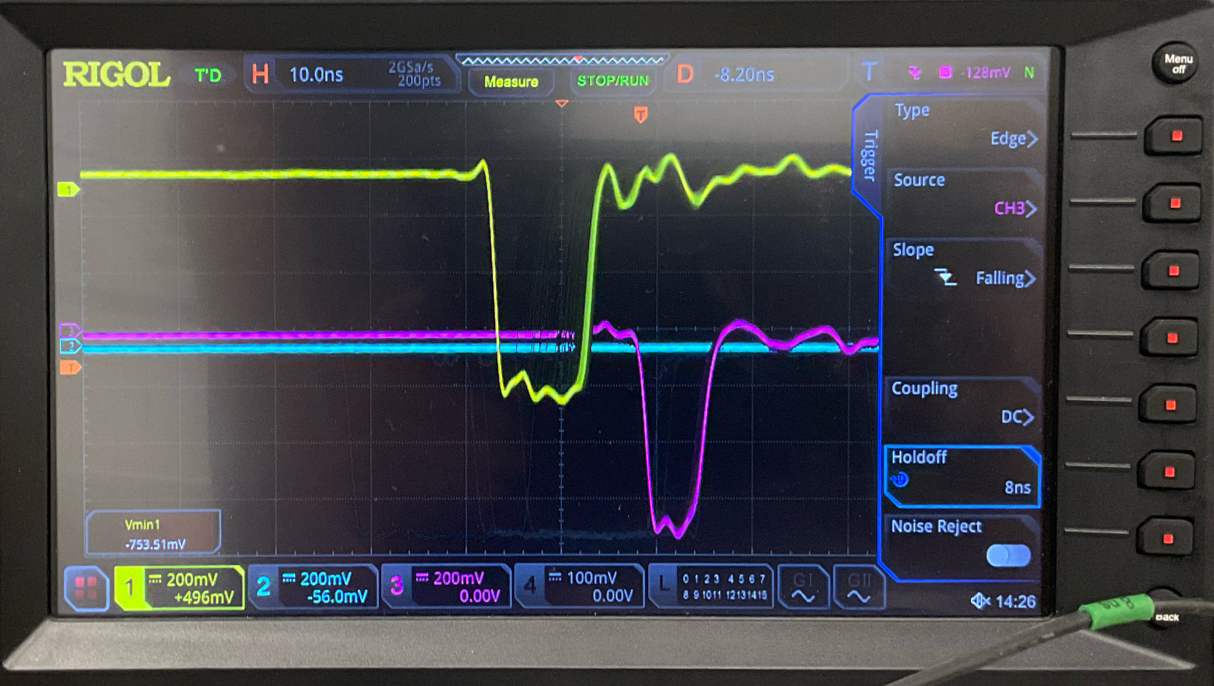
\includegraphics[width=0.48\linewidth]{VETO 4.jpeg}
    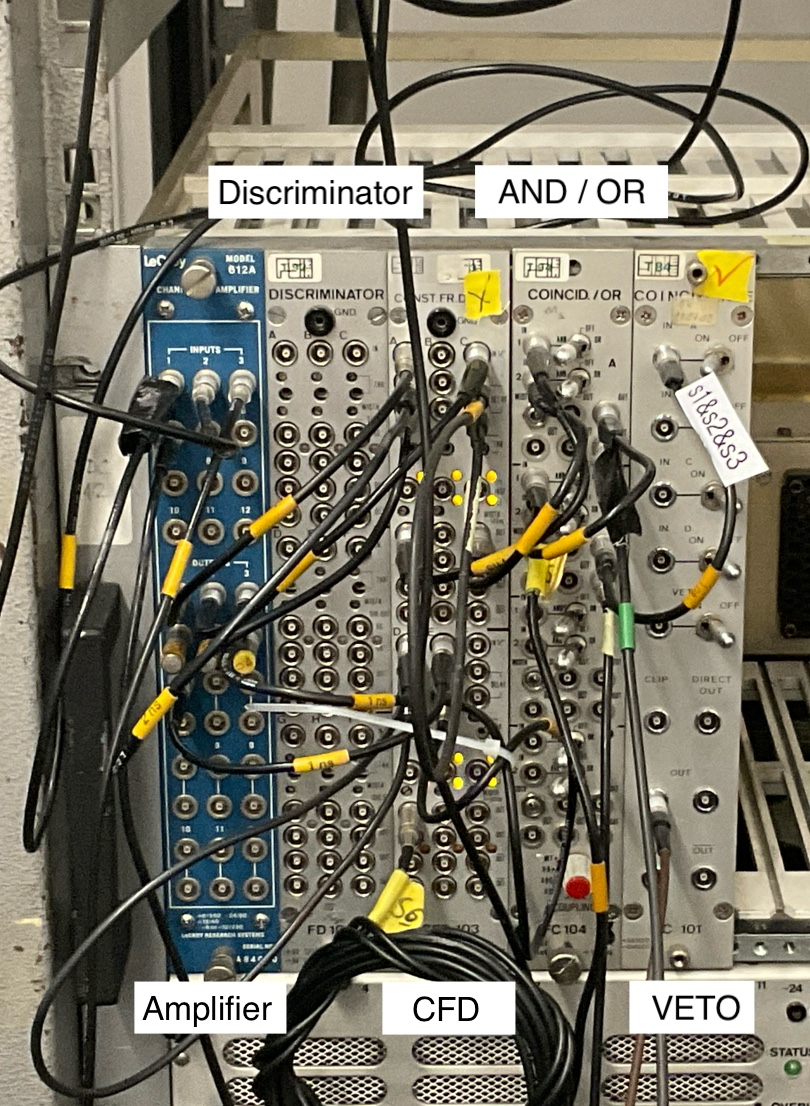
\includegraphics[width=0.28\linewidth]{START.jpeg}
    \caption{Left: Oscilloscope display showing the START signal (pink), which is generated only when S1, S2, and S3 (yellow) fire and the particle does not enter S4 (blue). Right: Final cabling setup for the START signal, showing the five modules used: signal amplifier, standard discriminator, constant fraction discriminator, AND/OR module, and VETO module.}
    \label{final}
\end{figure}

\subsubsection{STOP signal}


The STOP signal was defined by the coincidence of scintillators S6 and S7, placed downstream of the target at $\sim 135^\circ$ relative to the beam axis. Both detectors were connected to discriminators to convert the analog PMT pulses into logic signals. The two outputs were then fed into a coincidence unit to perform a logical AND operation:

\begin{equation*}
\text{STOP:} \quad \text{S6} \: \land \: \text{S7}.
\end{equation*}

Since the S6 and S7 signals had slightly different timing characteristics, the S7 signal was delayed and its logic width narrowed. This ensured that the output of the AND gate coincided precisely with the timing of S7, so that the STOP signal was generated at the moment of the S7 detection. Figure~\ref{STOPscope} illustrates this: the yellow trace corresponds to S6, the blue trace to S7, and the resulting violet signal represents the coincidence S6 $\&$ S7.

\begin{figure}[h]
\centering
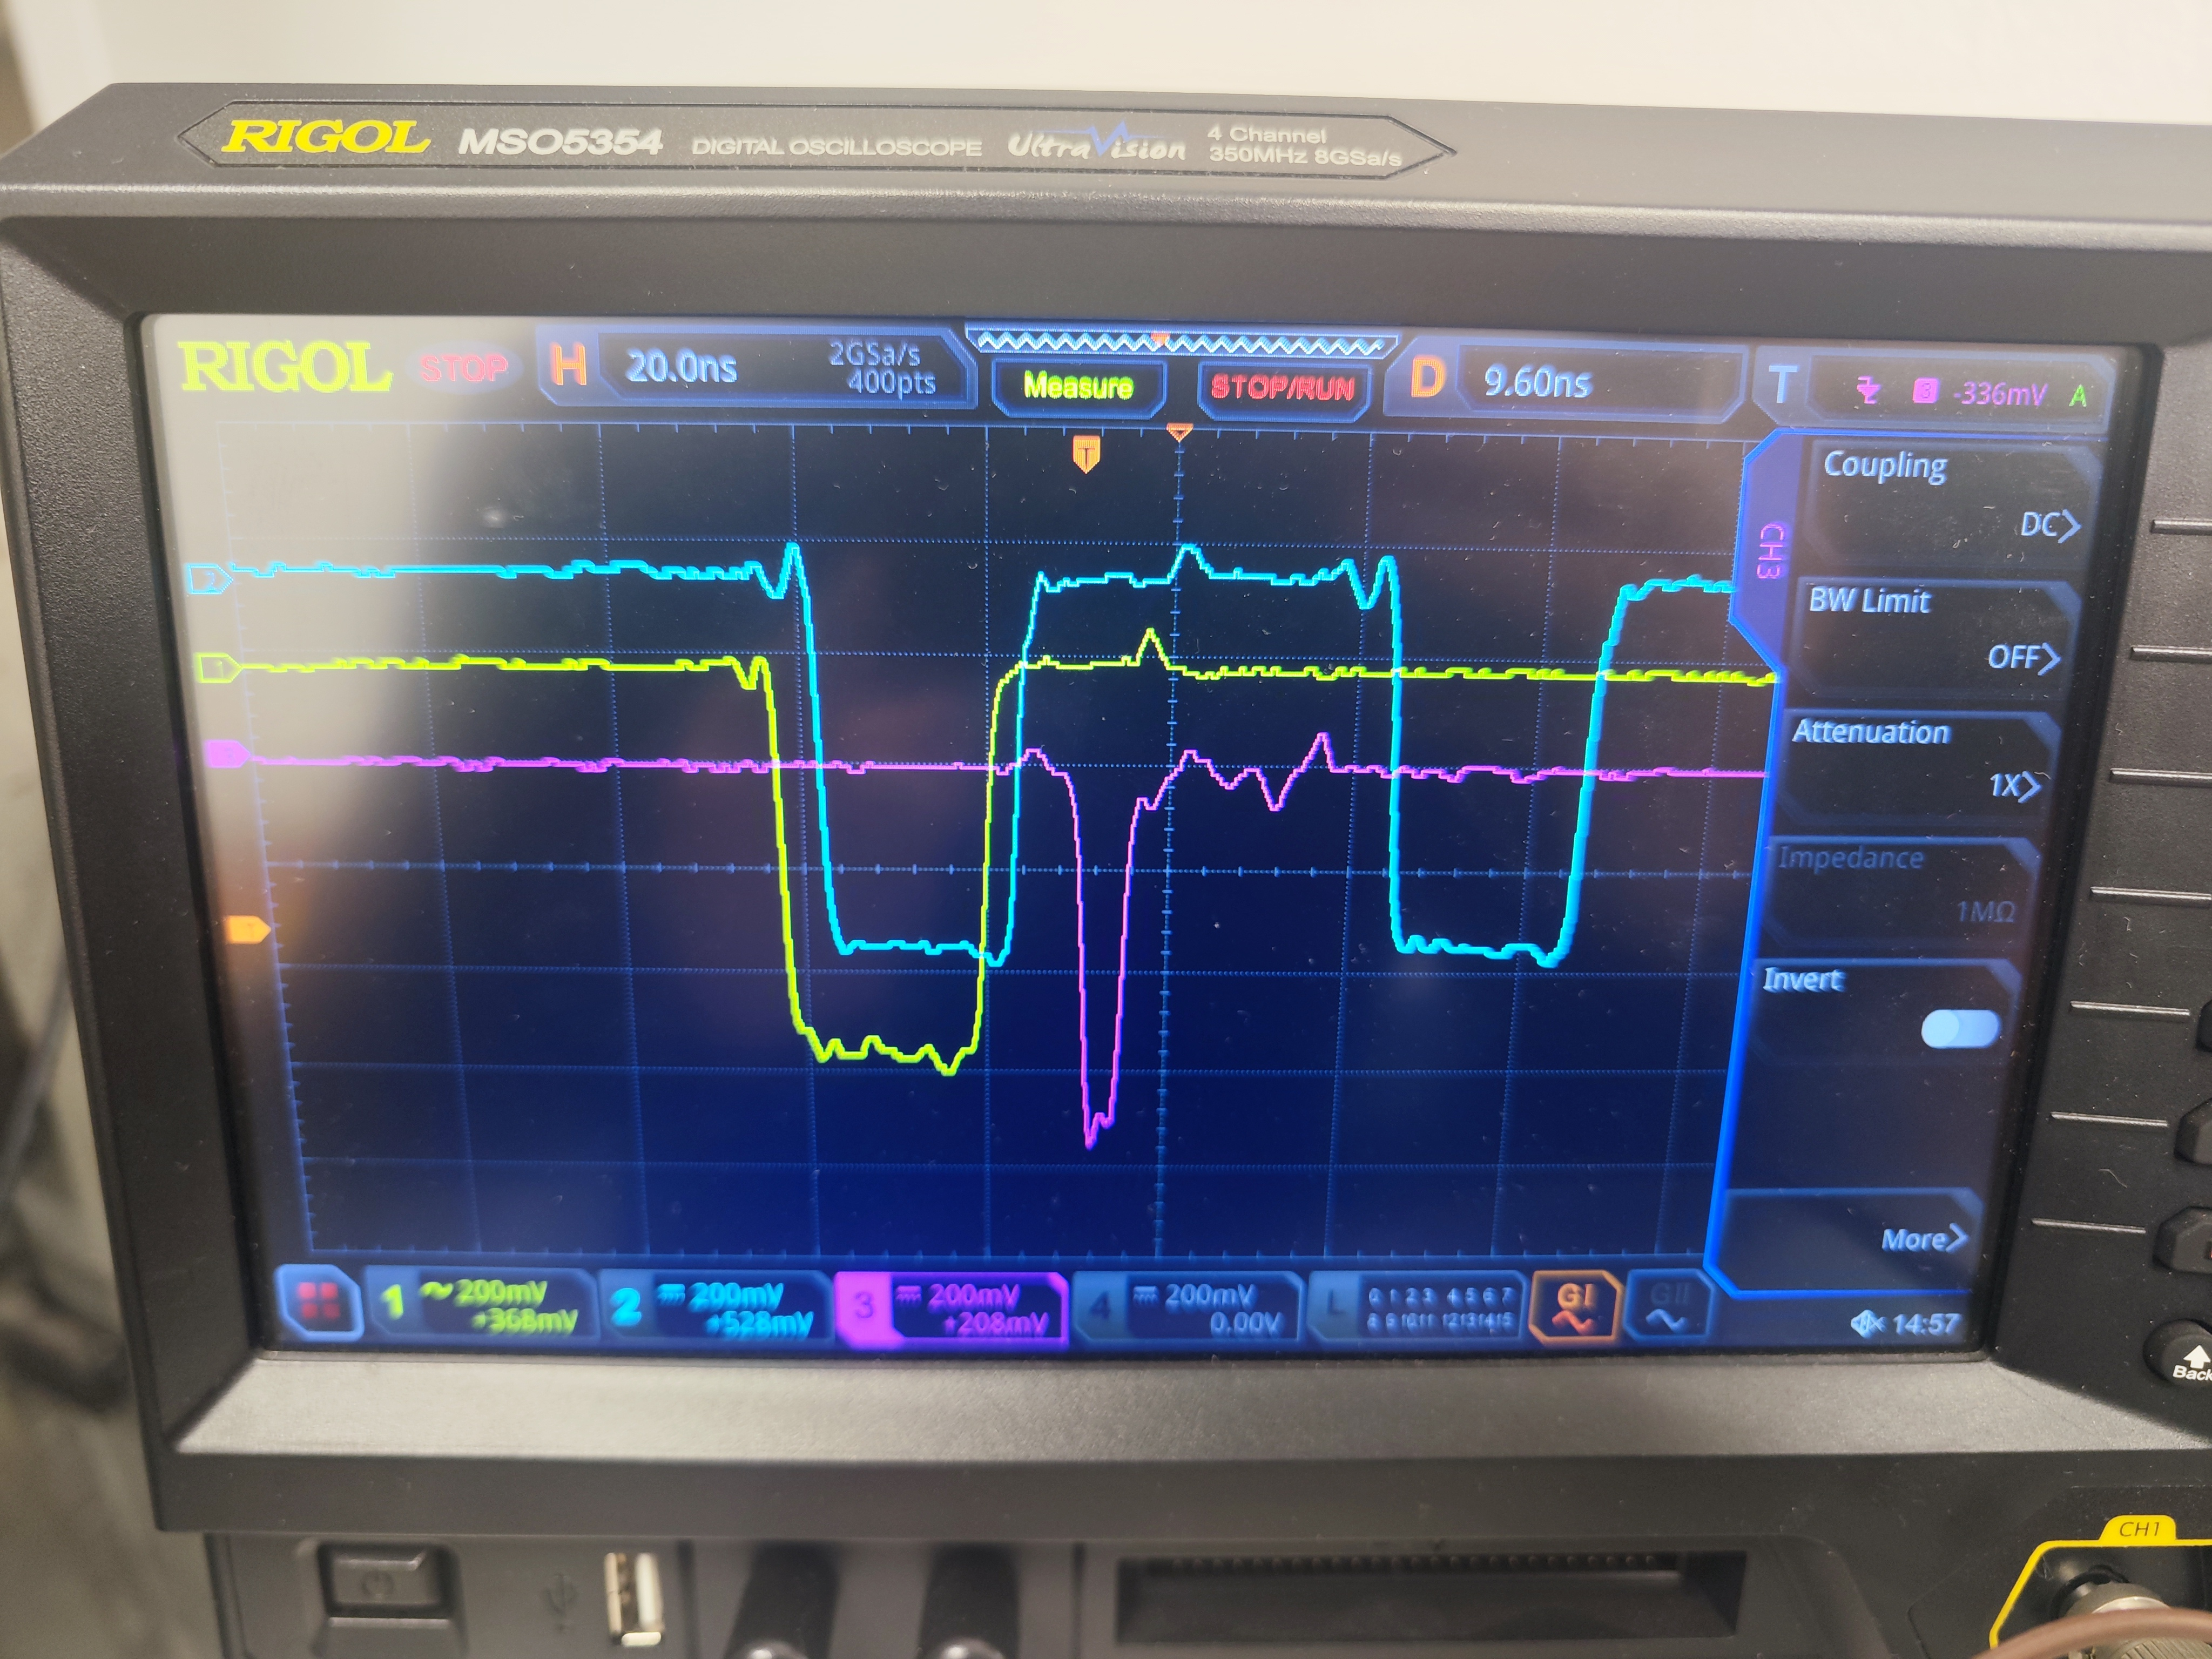
\includegraphics[width=0.48\linewidth]{S6S7.jpg}
\caption{Oscilloscope display of the STOP signal formation. Yellow: S6, blue: S7, violet: coincidence of S6 and S7.}
\label{STOPscope}
\end{figure}

In the original setup, two additional detectors were included for background suppression. Scintillator S5, positioned with a central hole in front of S6, could act as a veto to reject events where particles entered from non-vertical directions. Furthermore, a backup signal from scintillator S8 (mounted on S6) was used to further suppress hadronic background. The discriminator threshold of S8 was set to a higher value, so that only large-amplitude pulses, characteristic of hadronic interactions, produced an output. This veto condition ensured that events with unwanted hadron contributions were efficiently rejected.

However, in the present measurement, only the coincidence of S6 and S7 was actually used to define the STOP signal.
The resulting STOP logic pulse was then fed into the \texttt{DRIGGER} (delay module)input of the TAC module,
where it was combined with the START signal to measure the time difference between pion stop and positron detection.

\subsubsection{Time-to-Amplitude Converter (TAC)}

The time measurement in this experiment was performed using a Time-to-Amplitude Converter (TAC) module.
The TAC receives two logic inputs: the START signal (from the coincidence of S1, S2, and S3 in anti-coincidence with S4)
and the STOP signal (from the coincidence of S6 and S7).
Whenever a START signal arrives, the TAC begins charging a capacitor.
The charging is stopped as soon as the corresponding STOP signal is received at the \texttt{DTRIGGER} input.
The resulting voltage amplitude at the TAC output is therefore proportional to the time difference $\Delta t = t_{\text{STOP}} - t_{\text{START}}$.

\begin{figure}[h]
\centering
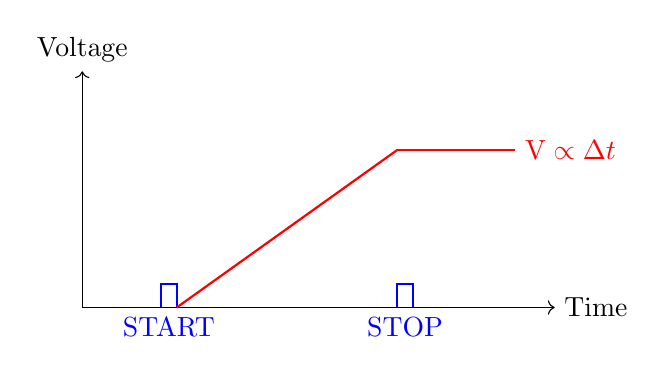
\begin{tikzpicture}[scale=1.0]
\draw[->] (0,0) -- (6,0) node[right]{Time};
\draw[->] (0,0) -- (0,3) node[above]{Voltage};

		% START pulse
		\draw[thick,blue] (1,0) -- (1,0.3) -- (1.2,0.3) -- (1.2,0);
		\node[blue,below] at (1.1,0) {START};

		% Charging
		\draw[thick,red] (1.2,0) -- (4,2);

		% STOP pulse
		\draw[thick,blue] (4,0) -- (4,0.3) -- (4.2,0.3) -- (4.2,0);
		\node[blue,below] at (4.1,0) {STOP};

		% Hold voltage
		\draw[thick,red] (4,2) -- (5.5,2);
        \node[right,red] at (5.5,2) {$\text{V} \propto \Delta t$};
\end{tikzpicture}
\caption{Working principle of the TAC: the capacitor charges between START and STOP signals, producing a voltage proportional to the time difference.}
\end{figure}

In this way, the decay time between the pion stopping in the target and the detection of the decay positron could be translated into an analog voltage.
This output was then processed further by the ADC module.

\subsubsection{Analog-to-Digital Converter (ADC) and data acquisition}

The analog output of the TAC was digitized using an Analog-to-Digital Converter (ADC).
The ADC module receives two inputs: the analog voltage from the TAC, and a logic GATE signal which defines the time window during which the conversion should take place.
When triggered, the ADC converts the analog amplitude into a digital number proportional to the measured decay time.

The digitized values were then transferred via USB to a dedicated Windows laptop in the control room,
which ran the \texttt{MAESTRO} data acquisition software.
This software accumulated the time spectra into histograms, displayed them in real time, and stored the data locally. And then data was used for later analysis.
In addition, calibration runs were performed in which the ADC digital values were compared with well-defined delay times, producing calibration histograms.
This time calibration allowed us to convert the raw ADC output into physical decay times, providing the basis for the analysis and lifetime fitting of the event–time spectra.
\subsection{Readout electronics summary}

\begin{figure}[ht]
\centering
% ---- SCALE THE ENTIRE TIKZ TO PAGE WIDTH ----
\resizebox{\textwidth}{!}{%
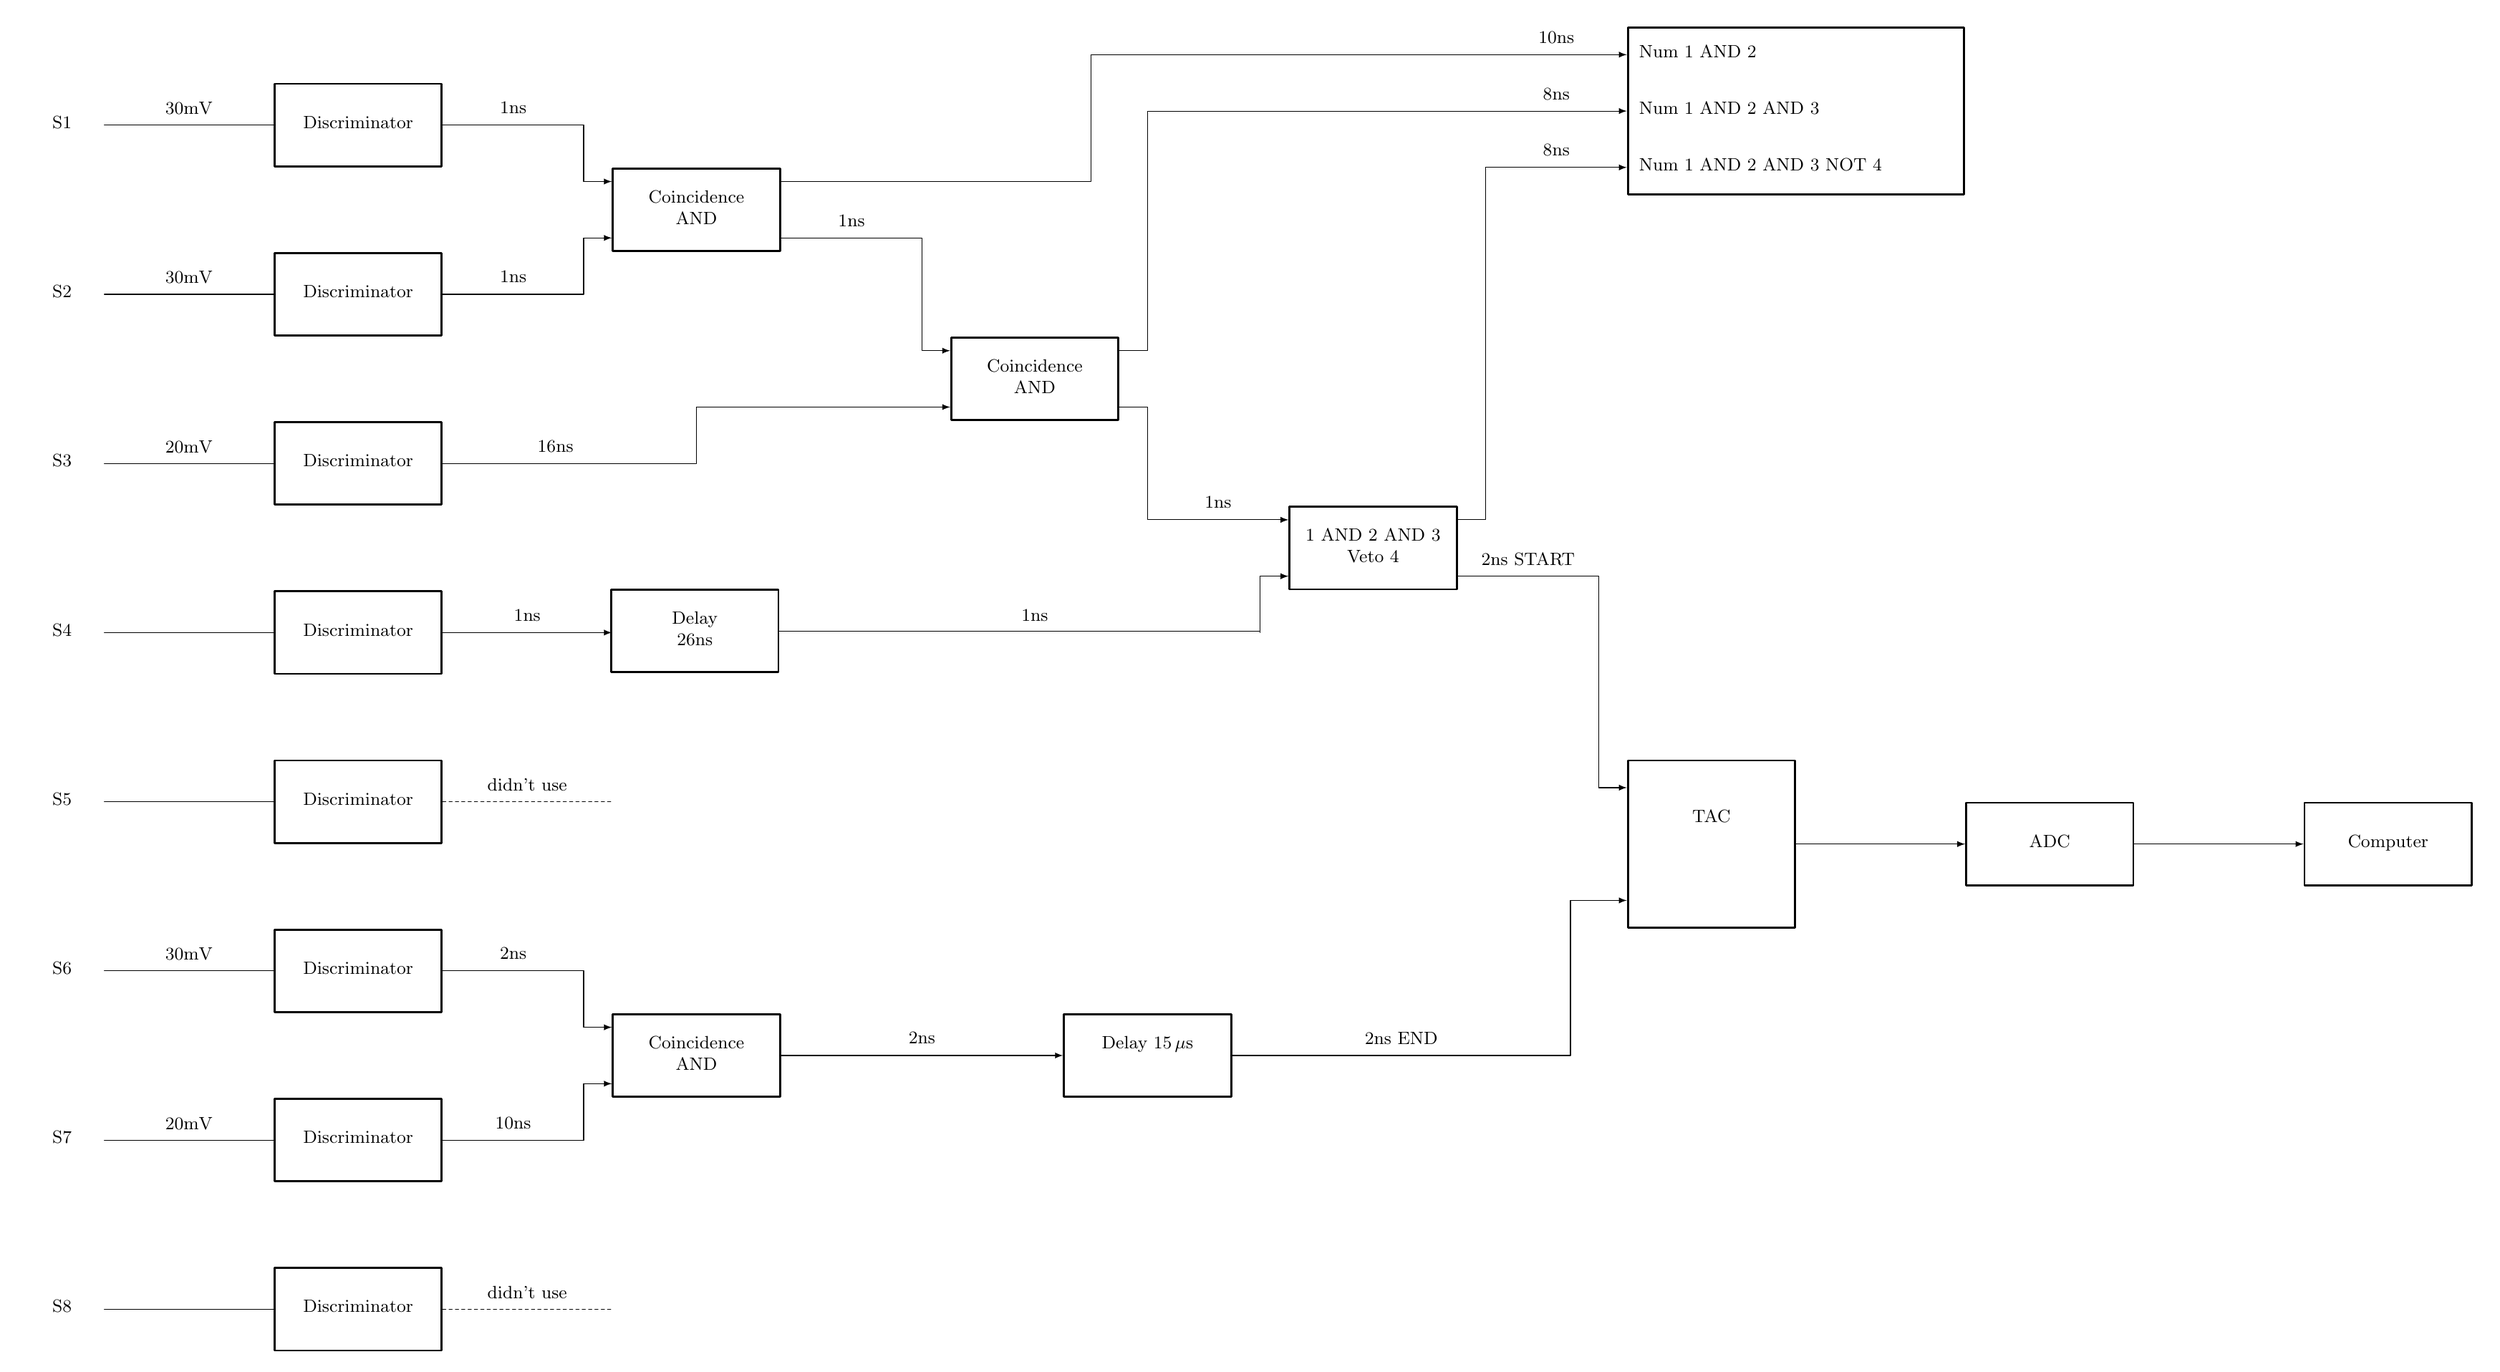
\begin{tikzpicture}[
=Latex,
line cap=round, line join=round,
every path/.style={line width=0.4pt},
every node/.style={font=\small,align=center,inner sep=4pt,transform shape}
]
% Paths, nodes and wires:
% \node[shape=rectangle, draw, line width=1pt, minimum width=2.215cm, minimum height=-0.035cm] at (1.125, 6){};
\node[shape=rectangle, draw, line width=1pt, minimum width=2.965cm, minimum height=1.465cm] at (1.5, 5.25){};
\node[shape=rectangle, draw, line width=1pt, minimum width=2.965cm, minimum height=1.465cm] at (1.5, 2.25){};
% \node[shape=rectangle, draw, line width=1pt, minimum width=2.215cm, minimum height=-0.035cm] at (1.654, 5.471){};
\node[shape=rectangle, draw, line width=1pt, minimum width=2.965cm, minimum height=1.465cm] at (1.5, -6.75){};
\node[shape=rectangle, draw, line width=1pt, minimum width=2.965cm, minimum height=1.465cm] at (1.5, -9.75){};
% \node[shape=rectangle, draw, line width=1pt, minimum width=2.215cm, minimum height=-0.035cm] at (1.125, -0){};
\node[shape=rectangle, draw, line width=1pt, minimum width=2.965cm, minimum height=1.465cm] at (1.5, -0.75){};
\node[shape=rectangle, draw, line width=1pt, minimum width=2.965cm, minimum height=1.465cm] at (1.5, -3.75){};
\node[shape=rectangle, draw, line width=1pt, minimum width=2.965cm, minimum height=1.465cm] at (1.5, -12.75){};
\node[shape=rectangle, draw, line width=1pt, minimum width=2.965cm, minimum height=1.465cm] at (1.5, -15.75){};
\node[shape=rectangle, minimum width=3.215cm, minimum height=0.715cm] at (1.5, 5.25){} node[anchor=north, align=center, text width=2.827cm, inner sep=6pt] at (1.5, 5.625){Discriminator};
\node[shape=rectangle, minimum width=3.215cm, minimum height=0.715cm] at (1.5, 2.25){} node[anchor=north, align=center, text width=2.827cm, inner sep=6pt] at (1.5, 2.625){Discriminator};
\node[shape=rectangle, minimum width=3.215cm, minimum height=0.715cm] at (1.5, -0.75){} node[anchor=north, align=center, text width=2.827cm, inner sep=6pt] at (1.5, -0.375){Discriminator};
\node[shape=rectangle, minimum width=3.215cm, minimum height=0.715cm] at (1.5, -3.75){} node[anchor=north, align=center, text width=2.827cm, inner sep=6pt] at (1.5, -3.375){Discriminator};
\node[shape=rectangle, minimum width=3.215cm, minimum height=0.715cm] at (1.5, -6.75){} node[anchor=north, align=center, text width=2.827cm, inner sep=6pt] at (1.5, -6.375){Discriminator};
\node[shape=rectangle, minimum width=3.215cm, minimum height=0.715cm] at (1.5, -9.75){} node[anchor=north, align=center, text width=2.827cm, inner sep=6pt] at (1.5, -9.375){Discriminator};
\node[shape=rectangle, minimum width=3.215cm, minimum height=0.715cm] at (1.5, -12.75){} node[anchor=north, align=center, text width=2.827cm, inner sep=6pt] at (1.5, -12.375){Discriminator};
\node[shape=rectangle, minimum width=3.215cm, minimum height=0.715cm] at (1.5, -15.75){} node[anchor=north, align=center, text width=2.827cm, inner sep=6pt] at (1.5, -15.375){Discriminator};
\draw (0, 5.25) -- (-3, 5.25);
\draw (0, 2.25) -- (-3, 2.25);
\draw (0, -0.75) -- (-3, -0.75);
\draw (0, -3.75) -- (-3, -3.75);
\draw (0, -6.75) -- (-3, -6.75);
\draw (0, -9.75) -- (-3, -9.75);
\draw (0, -12.75) -- (-3, -12.75);
\draw (0, -15.75) -- (-3, -15.75);
\node[shape=rectangle, minimum width=1.465cm, minimum height=0.715cm] at (-3.75, 5.25){} node[anchor=north, align=center, text width=1.077cm, inner sep=6pt] at (-3.75, 5.625){S1};
\node[shape=rectangle, minimum width=1.465cm, minimum height=0.715cm] at (-3.75, 2.25){} node[anchor=north, align=center, text width=1.077cm, inner sep=6pt] at (-3.75, 2.625){S2};
\node[shape=rectangle, minimum width=1.465cm, minimum height=0.715cm] at (-3.75, -0.75){} node[anchor=north, align=center, text width=1.077cm, inner sep=6pt] at (-3.75, -0.375){S3};
\node[shape=rectangle, minimum width=1.465cm, minimum height=0.715cm] at (-3.75, -3.75){} node[anchor=north, align=center, text width=1.077cm, inner sep=6pt] at (-3.75, -3.375){S4};
\node[shape=rectangle, minimum width=1.465cm, minimum height=0.715cm] at (-3.75, -6.75){} node[anchor=north, align=center, text width=1.077cm, inner sep=6pt] at (-3.75, -6.375){S5};
\node[shape=rectangle, minimum width=1.465cm, minimum height=0.715cm] at (-3.75, -9.75){} node[anchor=north, align=center, text width=1.077cm, inner sep=6pt] at (-3.75, -9.375){S6};
\node[shape=rectangle, minimum width=1.465cm, minimum height=0.715cm] at (-3.75, -12.75){} node[anchor=north, align=center, text width=1.077cm, inner sep=6pt] at (-3.75, -12.375){S7};
\node[shape=rectangle, minimum width=1.465cm, minimum height=0.715cm] at (-3.75, -15.75){} node[anchor=north, align=center, text width=1.077cm, inner sep=6pt] at (-3.75, -15.375){S8};
\node[shape=rectangle, draw, line width=1pt, minimum width=2.965cm, minimum height=1.465cm] at (7.5, 3.75){};
\node[shape=rectangle, minimum width=3.215cm, minimum height=1.09cm] at (7.5, 3.75){} node[anchor=north, align=center, text width=2.827cm, inner sep=6pt] at (7.5, 4.312){Coincidence\\AND};
\node[shape=rectangle, draw, line width=1pt, minimum width=2.965cm, minimum height=1.465cm] at (13.5, 0.75){};
\node[shape=rectangle, minimum width=3.215cm, minimum height=1.09cm] at (13.5, 0.75){} node[anchor=north, align=center, text width=2.827cm, inner sep=6pt] at (13.5, 1.312){Coincidence\\AND};
\node[shape=rectangle, draw, line width=1pt, minimum width=2.965cm, minimum height=1.465cm] at (7.471, -3.721){};
\node[shape=rectangle, minimum width=3.215cm, minimum height=1.09cm] at (7.471, -3.721){} node[anchor=north, align=center, text width=2.827cm, inner sep=6pt] at (7.471, -3.158){Delay\\26ns};
\draw[-latex] (3, -3.75) -- (6, -3.75);
\draw[dash pattern={on 1.6pt off 1.6pt}] (3, -6.75) -- (6, -6.75);
\node[shape=rectangle, draw, line width=1pt, minimum width=2.965cm, minimum height=1.465cm] at (7.5, -11.25){};
\node[shape=rectangle, minimum width=3.215cm, minimum height=1.09cm] at (7.5, -11.25){} node[anchor=north, align=center, text width=2.827cm, inner sep=6pt] at (7.5, -10.687){Coincidence\\AND};
\node[shape=rectangle, minimum width=2.465cm, minimum height=0.715cm] at (4.5, -6.5){} node[anchor=north, align=center, text width=2.077cm, inner sep=6pt] at (4.5, -6.125){didn't use};
\draw[dash pattern={on 1.6pt off 1.6pt}] (3, -15.75) -- (6, -15.75);
\node[shape=rectangle, minimum width=2.465cm, minimum height=0.715cm] at (4.5, -15.5){} node[anchor=north, align=center, text width=2.077cm, inner sep=6pt] at (4.5, -15.125){didn't use};
\node[shape=rectangle, minimum width=2.465cm, minimum height=0.715cm] at (-1.5, -12.5){} node[anchor=north, align=center, text width=2.077cm, inner sep=6pt] at (-1.5, -12.125){20mV};
\node[shape=rectangle, minimum width=2.465cm, minimum height=0.715cm] at (-1.5, -9.5){} node[anchor=north, align=center, text width=2.077cm, inner sep=6pt] at (-1.5, -9.125){30mV};
\node[shape=rectangle, minimum width=2.465cm, minimum height=0.715cm] at (-1.5, -0.5){} node[anchor=north, align=center, text width=2.077cm, inner sep=6pt] at (-1.5, -0.125){20mV};
\node[shape=rectangle, minimum width=2.465cm, minimum height=0.715cm] at (-1.5, 2.5){} node[anchor=north, align=center, text width=2.077cm, inner sep=6pt] at (-1.5, 2.875){30mV};
\node[shape=rectangle, minimum width=2.465cm, minimum height=0.715cm] at (-1.5, 5.5){} node[anchor=north, align=center, text width=2.077cm, inner sep=6pt] at (-1.5, 5.875){30mV};
\node[shape=rectangle, minimum width=2.465cm, minimum height=0.715cm] at (4.5, -3.5){} node[anchor=north, align=center, text width=2.077cm, inner sep=6pt] at (4.5, -3.125){1ns};
\draw[-latex] (3, 5.25) -- (5.5, 5.25) -| (5.5, 4.25) -- (6, 4.25);
\draw[-latex] (3, 2.25) -- (5.5, 2.25) -| (5.5, 3.25) -- (6, 3.25);
\node[shape=rectangle, minimum width=2.465cm, minimum height=0.715cm] at (4.25, 2.5){} node[anchor=north, align=center, text width=2.077cm, inner sep=6pt] at (4.25, 2.875){1ns};
\node[shape=rectangle, minimum width=2.465cm, minimum height=0.715cm] at (4.25, 5.5){} node[anchor=north, align=center, text width=2.077cm, inner sep=6pt] at (4.25, 5.875){1ns};
\node[shape=rectangle, minimum width=2.465cm, minimum height=0.715cm] at (5, -0.5){} node[anchor=north, align=center, text width=2.077cm, inner sep=6pt] at (5, -0.125){16ns};
\draw[-latex] (3, -0.75) -- (7.5, -0.75) -| (7.5, 0.25) -- (12, 0.25);
\draw[-latex] (9, 3.25) -- (11.5, 3.25) -| (11.5, 1.25) -- (12, 1.25);
\node[shape=rectangle, minimum width=2.465cm, minimum height=0.715cm] at (10.25, 3.5){} node[anchor=north, align=center, text width=2.077cm, inner sep=6pt] at (10.25, 3.875){1ns};
\draw[-latex] (3, -9.75) -- (5.5, -9.75) -| (5.5, -10.75) -- (6, -10.75);
\draw[-latex] (3, -12.75) -- (5.5, -12.75) -| (5.5, -11.75) -- (6, -11.75);
\node[shape=rectangle, minimum width=2.465cm, minimum height=0.715cm] at (4.25, -12.5){} node[anchor=north, align=center, text width=2.077cm, inner sep=6pt] at (4.25, -12.125){10ns};
\node[shape=rectangle, minimum width=2.465cm, minimum height=0.715cm] at (4.25, -9.5){} node[anchor=north, align=center, text width=2.077cm, inner sep=6pt] at (4.25, -9.125){2ns};
\node[shape=rectangle, draw, line width=1pt, minimum width=2.965cm, minimum height=1.465cm] at (19.5, -2.25){};
\node[shape=rectangle, minimum width=3.215cm, minimum height=1.09cm] at (19.5, -2.25){} node[anchor=north, align=center, text width=2.827cm, inner sep=6pt] at (19.5, -1.687){1 AND 2 AND 3\\Veto 4};
\draw[-latex] (8.971, -3.721) -| (17.5, -3.75) -| (17.5, -2.75) -- (18, -2.75);
\draw[-latex] (15, 0.25) -- (15.5, 0.25) -| (15.5, -1.75) -- (18, -1.75);
\node[shape=rectangle, draw, line width=1pt, minimum width=2.965cm, minimum height=1.465cm] at (15.5, -11.25){};
\node[shape=rectangle, minimum width=3.215cm, minimum height=1.09cm] at (15.5, -11.25){} node[anchor=north, align=center, text width=2.827cm, inner sep=6pt] at (15.5, -10.687){Delay $15\,\mu\text{s}$};
\draw[-latex] (9, -11.25) -- (14, -11.25);
\node[shape=rectangle, minimum width=2.465cm, minimum height=0.715cm] at (11.5, -11){} node[anchor=north, align=center, text width=2.077cm, inner sep=6pt] at (11.5, -10.625){2ns};
\node[shape=rectangle, minimum width=2.465cm, minimum height=0.715cm] at (13.5, -3.5){} node[anchor=north, align=center, text width=2.077cm, inner sep=6pt] at (13.5, -3.125){1ns};
\node[shape=rectangle, minimum width=2.465cm, minimum height=0.715cm] at (16.75, -1.5){} node[anchor=north, align=center, text width=2.077cm, inner sep=6pt] at (16.75, -1.125){1ns};
\node[shape=rectangle, draw, line width=1pt, minimum width=2.965cm, minimum height=2.965cm] at (25.5, -7.5){};
\draw[-latex] (17, -11.25) -- (23, -11.25) -| (23, -8.5) -- (24, -8.5);
\draw[-latex] (21, -2.75) -- (23.5, -2.75) -- (23.5, -6.5) -- (24, -6.5);
\node[shape=rectangle, minimum width=2.465cm, minimum height=0.715cm] at (20, -11){} node[anchor=north, align=center, text width=2.077cm, inner sep=6pt] at (20, -10.625){2ns END};
\node[shape=rectangle, minimum width=2.465cm, minimum height=0.715cm] at (22.25, -2.5){} node[anchor=north, align=center, text width=2.077cm, inner sep=6pt] at (22.25, -2.125){2ns START};
\node[shape=rectangle, minimum width=3.215cm, minimum height=1.59cm] at (25.5, -7.5){} node[anchor=north, align=center, text width=2.827cm, inner sep=6pt] at (25.5, -6.688){TAC};
\draw[-latex] (27, -7.5) -- (30, -7.5);
\node[shape=rectangle, draw, line width=1pt, minimum width=2.965cm, minimum height=1.465cm] at (31.5, -7.5){};
\node[shape=rectangle, minimum width=3.215cm, minimum height=0.715cm] at (31.5, -7.5){} node[anchor=north, align=center, text width=2.827cm, inner sep=6pt] at (31.5, -7.125){ADC};
\draw[-latex] (33, -7.5) -- (36, -7.5);
\node[shape=rectangle, draw, line width=1pt, minimum width=2.965cm, minimum height=1.465cm] at (37.5, -7.5){};
\node[shape=rectangle, minimum width=3.215cm, minimum height=0.715cm] at (37.5, -7.5){} node[anchor=north, align=center, text width=2.827cm, inner sep=6pt] at (37.5, -7.125){Computer};
\node[shape=rectangle, draw, line width=1pt, minimum width=5.965cm, minimum height=2.965cm] at (27, 5.5){};
\draw[-latex] (21, -1.75) -- (21.5, -1.75) -- (21.5, 4.5) -- (24, 4.5);
\draw[-latex] (15, 1.25) -- (15.5, 1.25) -| (15.5, 5.5) -- (24, 5.5);
\draw[-latex] (9, 4.25) -- (14.5, 4.25) -| (14.5, 6.5) -- (24, 6.5);
\node[shape=rectangle, minimum width=3.215cm, minimum height=0.715cm] at (25.625, 6.5){} node[anchor=north west, align=left, text width=2.827cm, inner sep=6pt] at (24, 6.875){Num 1 AND 2};
\node[shape=rectangle, minimum width=5.715cm, minimum height=0.715cm] at (26.875, 5.5){} node[anchor=north west, align=left, text width=5.327cm, inner sep=6pt] at (24, 5.875){Num 1 AND 2 AND 3};
\node[shape=rectangle, minimum width=5.715cm, minimum height=0.715cm] at (26.875, 4.5){} node[anchor=north west, align=left, text width=5.327cm, inner sep=6pt] at (24, 4.875){Num 1 AND 2 AND 3 NOT 4};
\node[shape=rectangle, minimum width=2.465cm, minimum height=0.715cm] at (22.75, 4.75){} node[anchor=north, align=center, text width=2.077cm, inner sep=6pt] at (22.75, 5.125){8ns};
\node[shape=rectangle, minimum width=2.465cm, minimum height=0.715cm] at (22.75, 5.75){} node[anchor=north, align=center, text width=2.077cm, inner sep=6pt] at (22.75, 6.125){8ns};
\node[shape=rectangle, minimum width=2.465cm, minimum height=0.715cm] at (22.75, 6.75){} node[anchor=north, align=center, text width=2.077cm, inner sep=6pt] at (22.75, 7.125){10ns};
% ==== your code to here ====
\end{tikzpicture}
}% end resizebox
\caption{In this layout, the entire trigger logic is presented, showing all implemented delays and electronic modules.}
\end{figure}

\section{Relevant parameters}

To optimize the beam parameters, we adjusted the dipole magnets (ASM), quadrupole magnets (QSL), and collimators (FSL), thereby tuning the beam momentum and focusing (see Figure \ref{piM1}).\\
During the experiment, counter modules were used to monitor the trigger rates of different detector combinations.
These counters directly displayed the counts from specific logic coincidence signals on digital displays, serving as important diagnostic tools. The values were read off manually and recorded in the experimental logbook. By recording 10-second counts while varying the beam parameters, we identified the optimal beam configuration.\\
%Under these conditions, the particle spectrum exhibited two distinct peaks, corresponding to pions and muons, confirming proper focusing and collimation of the beam at the target. (I don't know where this fits in. Just leave it a comment for now.)

%This following lines seem to be redundant. I love them here commented just in case!!

%\section{Relevant Parameters}

%In order to successfully perform the experiment, several experimental parameters had to be adjusted and optimized.
%These parameters can be grouped into two categories:
%(1) the beamline configuration, which determines how the secondary beam is guided and stopped in the target, and
%(2) the electronics and readout chain, which define how detector signals are processed, combined into logic triggers, and recorded. Does this fit in this section?
%For the beamline, the relevant settings include the beam direction, focus, and momentum, all of which are controlled by the currents in the dipole and quadrupole magnets.
%For the electronics, the relevant parameters include the configuration of logic coincidences, discriminator thresholds, and counter or TDC connections.
In the following subsections, these parameters and their optimization are discussed in detail.

The beam was optimized such that the largest fraction of particles would hit the target. After achieving that, the beam momentum was optimized so that the biggest fraction of Pions got stopped in the target. The following beam characteristics are altered in this process:



\begin{itemize}
\item Direction
\item Focus
\item Momentum
\end{itemize}


\subsection{Beam-Direction}
Changing the direction of the beam can be done by increasing the current, and therefore increasing the magnetic fields, in the ASM12 magnet.\\
On the other hand, the focus of the beam was changed by varying the currents through the quadrupole magnet at the end of the beamline. This process could be automated. A computer program would automatically vary the current in a selected magnet in a predefined range. The signal of $1 \land 2 \land 3 $  needed to be connected to the computer for that. After sweeping through the given range, the current resulting in the most incidents would be chosen for that magnet.\\

\subsection{Beam-Momentum}

With changing the beam momentum, goal was to maximize the following ratios:

\[
R_1 = \frac{S1 \land S2 \land S3}{S1 \land S2}, \qquad
R_2 = \frac{S1 \land S2 \land S3 \land \lnot S4}{S1 \land S2 \land S3}.
\]

A high value of $R_1$ indicates that particles passing through S1 and S2 were also efficiently stopped in the target (S3), while a high value of $R_2$ ensures that through-going particles (background detected in S4) were effectively suppressed.

By varying the current through magnet ASM11 we selected for a specific momentum. To ensure all the other beam parameters wouldn't need calibration after changing the beam momentum, changes were done to all other magnets in the beam line simultaneously. To make this process easier, we started with an arbitrary currant 115.09A and multiplied all currents by a percentage. This process was done manually. The relevant signals from the read out chain were connected to a counter module and the counts where read of from there. \\
With 115.09 A being the starting value and the maximum at 102.5\% , the value 118 A was used in magnet ASM11, resulting in a beam momentum of 125MeV.

\begin{table}[]
\centering
\begin{tabular}{|l|l|l|l|l|l|}
\hline
Scale Factor & \#$1 \land 2$ &\# $1 \land 2 \land 3$ &\# $1 \land 2 \land 3 \land \Bar{4}$ &\# $\frac{1 \land 2 \land 3}{1 \land 2}$ & \#$\frac{1 \land 2 \land 3 \land \Bar{4}}{1 \land 2 \land 3}$ \\ \hline
0.75         & 826847      & 118684              & 6684                              & 0.14353804                            & 0.05631762                  \\ \hline
0.775        & 888721      & 128308              & 6795                              & 0.14437377                            & 0.05295851                  \\ \hline
0.8          & 960890      & 142085              & 7092                              & 0.14786812                            & 0.04991378                  \\ \hline
0.82         & 1008356     & 147375              & 7191                              & 0.14615374                            & 0.04879389                  \\ \hline
0.825        & 1016697     & 151792              & 7787                              & 0.14929915                            & 0.05130046                  \\ \hline
0.825        & 1045996     & 156932              & 8349                              & 0.15003117                            & 0.05320139                  \\ \hline
0.83         & 1020359     & 150034              & 9449                              & 0.1470404                             & 0.06297906                  \\ \hline
0.84         & 1040370     & 159290              & 10008                             & 0.15310899                            & 0.0628288                   \\ \hline
0.85         & 1032629     & 153300              & 9090                              & 0.14845603                            & 0.0592955                   \\ \hline
0.86         & 1097785     & 168036              & 9544                              & 0.15306822                            & 0.05679735                  \\ \hline
0.875        & 1101474     & 162101              & 6670                              & 0.14716734                            & 0.04114719                  \\ \hline
0.9          & 1169897     & 169145              & 6195                              & 0.1445811                             & 0.03662538                  \\ \hline
0.91         & 1155294     & 173765              & 6464                              & 0.1504076                             & 0.03719967                  \\ \hline
0.925        & 1225705     & 174450              & 6097                              & 0.14232625                            & 0.03494984                  \\ \hline
0.95         & 1341656     & 189377              & 6226                              & 0.14115168                            & 0.03287622                  \\ \hline
0.975        & 1457506     & 208360              & 7496                              & 0.14295653                            & 0.0359762                   \\ \hline
1            & 1553505     & 243622              & 35247                             & 0.15682087                            & 0.14467905                  \\ \hline
1.01         & 1424164     & 222431              & 33760                             & 0.15618356                            & 0.15177741                  \\ \hline
1.02         & 1583714     & 259261              & 42526                             & 0.16370443                            & 0.16402776                  \\ \hline
\bf{1.025}   & \bf{1620348}     & \bf{206946}              & \bf{37848}                             & \bf{0.12771701}                            & \bf{0.18288829}                  \\ \hline
1.03         & 1591077     & 262514              & 34584                             & 0.16499139                            & 0.13174155                  \\ \hline
1.04         & 1653158     & 276412              & 23849                             & 0.16720241                            & 0.08628062                  \\ \hline
1.05         & 1775255     & 297356              & 12494                             & 0.16750044                            & 0.04201698                  \\ \hline
1.075        & 1834409     & 308965              & 8880                              & 0.16842754                            & 0.02874112                  \\ \hline
1.1          & 1982114     & 335649              & 8678                              & 0.1693389                             & 0.02585439                  \\ \hline
\end{tabular}
\caption{Table of the measurements taken for optimizing the beam momentum with the maximum at 102.5\%.}
\end{table}



\begin{figure*}
\centering
\begin{subfigure}[b]{0.45\textwidth}
\centering
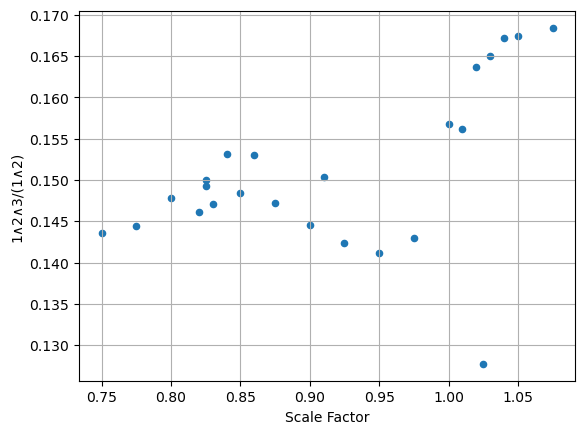
\includegraphics[width=\textwidth]{beam_optimization_1.png}
\caption{}

\end{subfigure}
    \hfill
    \begin{subfigure}[b]{0.45\textwidth}
        \centering
        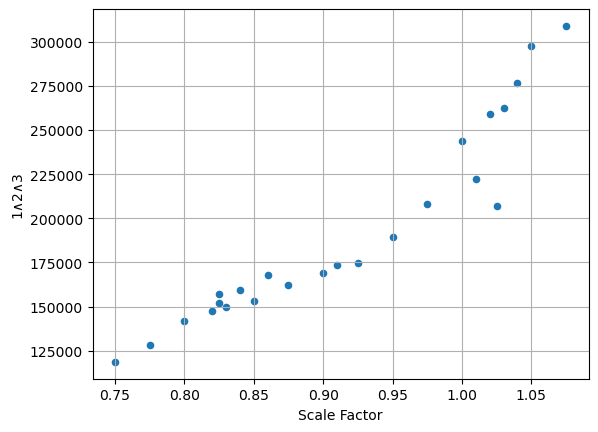
\includegraphics[width=\textwidth]{beam_optimization_2.png}
        \caption{}

    \end{subfigure}
    \vskip\baselineskip
    \begin{subfigure}[b]{0.45\textwidth}
        \centering
        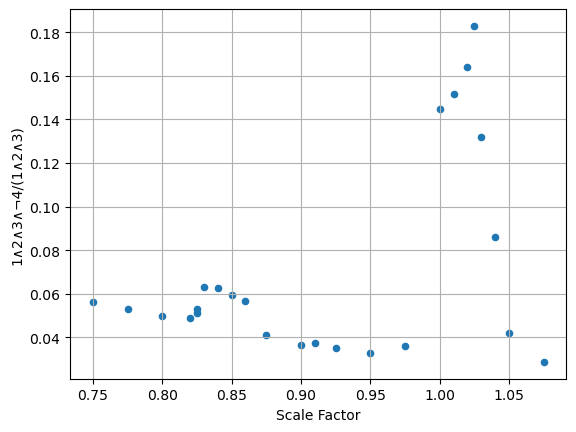
\includegraphics[width=\textwidth]{beam_optimization_3.png}
        \caption{}

    \end{subfigure}
    \hfill
    \begin{subfigure}[b]{0.45\textwidth}
        \centering
        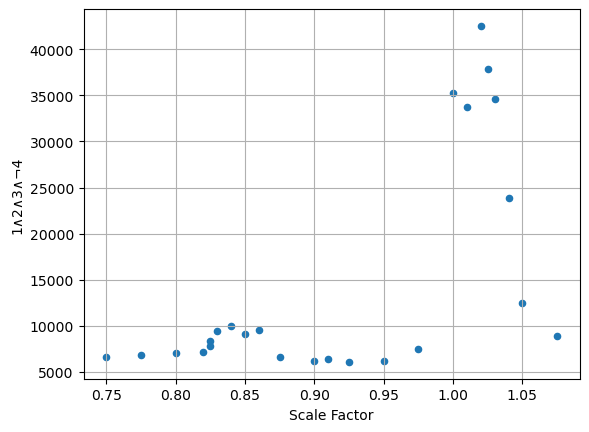
\includegraphics[width=\textwidth]{beam_optimization_4.png}
        \caption{}

    \end{subfigure}
    \caption{Percentages of current plotted against the resulting counts from which the beam momentum would be chosen by taking the maximum in figure d or minimum in figure c.}
\end{figure*}


\subsection{Electronics and Readout Chain Parameters}

The setup of the electronics and readout chain is described in Section~\ref{Electronics and triger logic}.

Here we only summarize the adjustable parameters that were relevant for data taking and optimization:

\begin{itemize}

\item \textbf{Discriminator thresholds:}

S1, S2, S4, and S6 were set to 30\,mV, while S3 and S7 were set to 20\,mV.

The lower thresholds for S3 and S7 were chosen to improve the timing response, since these detectors were used as start and stop signals, respectively

\item \textbf{Coincidence logic:}

Different logical combinations were used depending on the purpose:

$1 \land 2$ (beam intensity),

$1 \land 2 \land 3$ (particles reaching the target),

$1 \land 2 \land 3 \land \bar{4}$ (particles stopped in the target).

$6\land 7$  (stop signal positrons from muon decay).

\item \textbf{Delay of signals:}

Precise timing alignment between detectors was achieved by inserting signal delays.

\end{itemize}

\begin{itemize}
\item S3 was delayed by 16\,ns and combined in coincidence with S1 and S2.

This ensured that the start signal was consistently defined by S3.

\item S4 was passed through a 26\,ns delay module and then used as a veto signal in coincidence with S1, S2, and S3.

\item S6 was connected with a 2\,ns signal cable, and S7 with a 10\,ns signal cable, before being combined in coincidence.

This timing adjustment ensured that the stop signal was reliably defined by S7.

\item \textbf{Counting time window:}

During beam optimization, counts were recorded over a 10\,s interval to obtain reliable statistics.

\end{itemize}

In summary, the relevant parameters in the electronics chain were the discriminator thresholds, the choice of logic coincidences, the delay of signals, the counting time window, and the START/STOP signal definitions for the TDC.

\section{Simulation}


\subsection{Motivation}
In order to determine the optimal incident pion momentum that maximizes the probability of pions stopping inside the main target scintillator detector (S3).
A simulation was carried out using G4Beamline, based on the Geant4 framework, with the detector geometry and beam conditions of the real experiment, to produce an intuitive graphic demonstration. 

\subsection{Geometry and Materials}
The simulated setup included four scintillator detectors along the beamline (S1–S4), a 75 mm long plastic buffer, and three angled scintillators (S5–S7) with the same setup in the real experiment as shown in Figure 13:
Beamline scintillators and buffer: The distance between S1 and S2 is 133mm, the distance between S2 and S3 is 553mm, the distance between S3 and the buffer is 119mm, and the distance between S3 and S4 is 661mm.
\begin{figure}[h]
\centering
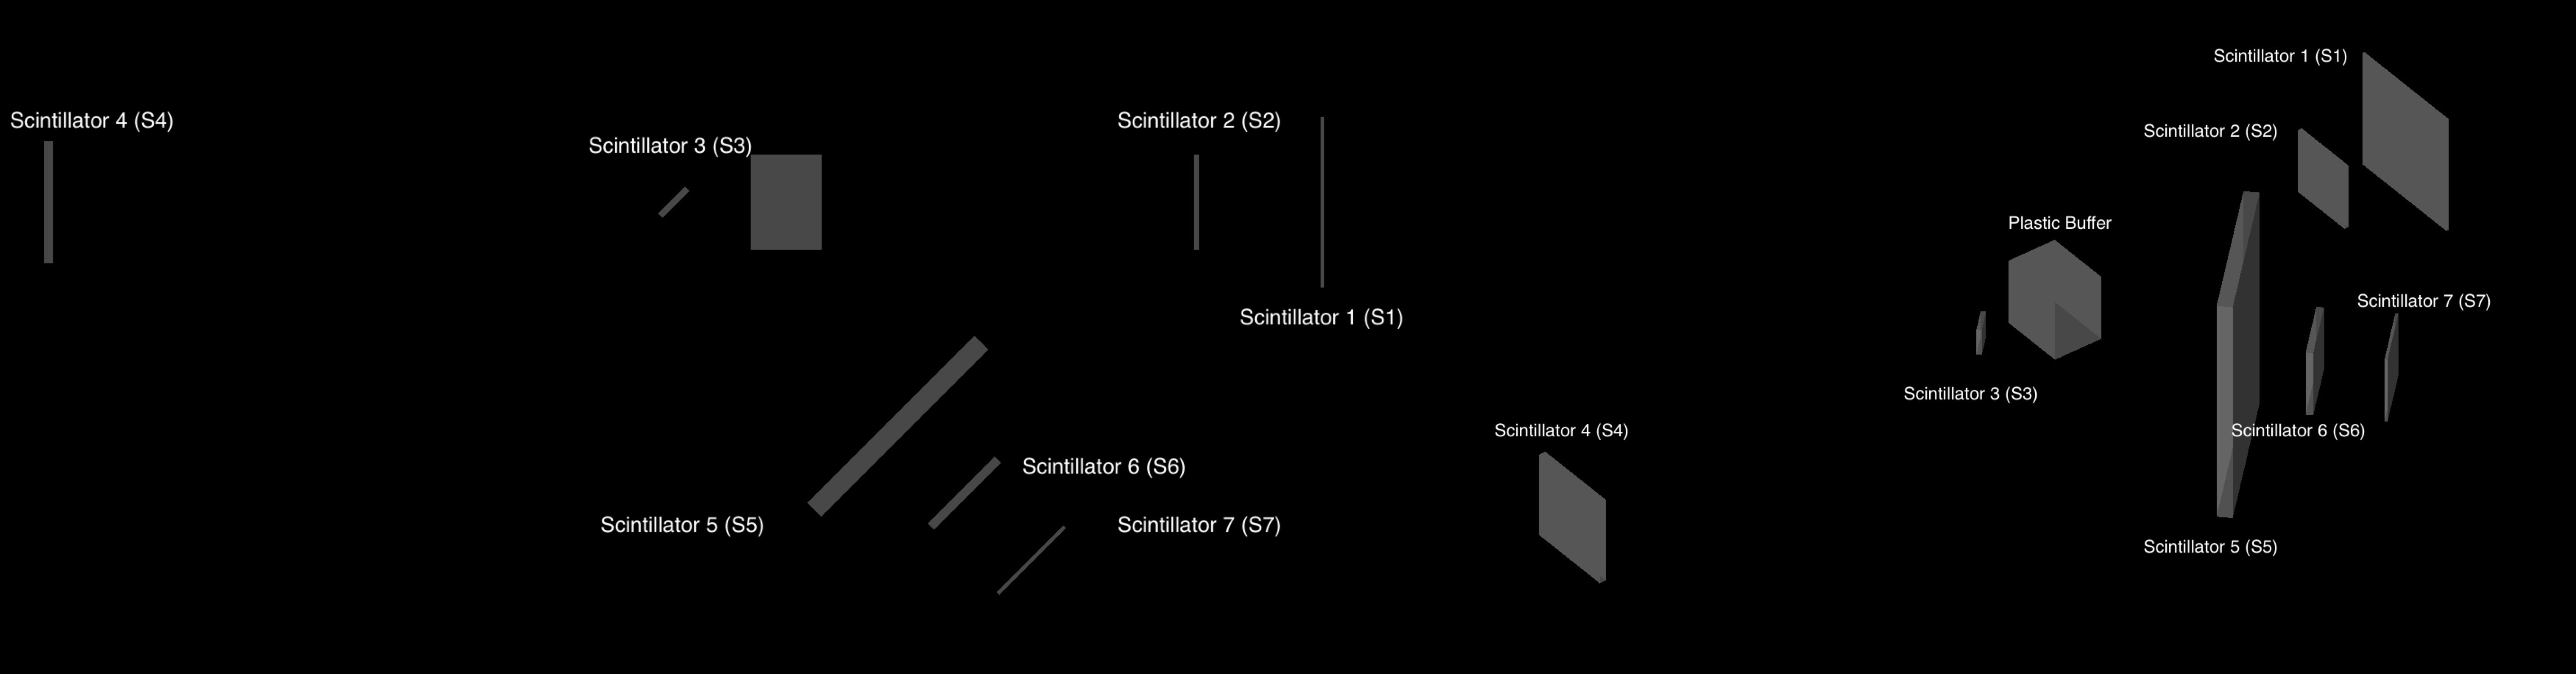
\includegraphics[width=0.70\linewidth]{1setup.JPEG}
\caption{Simulation SetUp}
\label{STOPscope}
\end{figure}

Angled scintillators: S3, S5, S6, and S7 were placed by rotating 135° relative to the beam axis to detect decay products. The distances from S3 to S5, S6, and S7 were 335 mm, 422 mm, and 535 mm, respectively.

All scintillators were modeled with the same size and shape as in the real setup, as shown in the table in the above session. The material was defined as POLYSTYRENE, with a density similar to that of the stopping power of the real scintillators and buffer.

\subsection{Beam Setup}
The following particles are considered in the simulation: Pions and anti-pions (red tracks), Muons and anti-muons (blue tracks), Electrons and positrons (green tracks), Protons and anti-protons (yellow tracks). 

\subsection{Results}
The outcome of different beam momentums are simulated, with momentum ranging from 300 MeV/c to 125 MeV/c. 

300 MeV/c: as shown in the figure 14, the pion (Red) barely stopped inside the target, and it could be observed that the hadronic interactions result in protons (yellow) mostly occurred in forward direction rather than backward(Figure 14).

\begin{figure}[h]
\centering
\includegraphics[width=0.70\linewidth]{300MeV.PNG}
\caption{Simulation with 300MeV/c momentum}
\label{STOPscope}
\end{figure}

150 MeV/c: A small fraction of pions began to get stopped in the target, and fewer hadronic interactions were observed(Figure 15).

\begin{figure}[h]
\centering
\includegraphics[width=0.70\linewidth]{150MeV.PNG}
\caption{Simulation with 150MeV/c momentum}
\label{STOPscope}
\end{figure}

139 MeV/c: More pions get stopped inside S3(Figure 16). 

\begin{figure}[h]
\centering
\includegraphics[width=0.70\linewidth]{139MeV.PNG}
\caption{Simulation with 139MeV/c momentum}
\label{STOPscope}
\end{figure}

130 MeV/c: A clear increase in stopping probability within S3, with good statistics for analysis(Figure 17).

\begin{figure}[h]
\centering
\includegraphics[width=0.70\linewidth]{130MeV.PNG}
\caption{Simulation with 130MeV/c momentum}
\label{STOPscope}
\end{figure}

125 MeV/c: Many pions stopped in the target as observed, approximately the same momentum chosen in the real experiment(Figure 18).

\begin{figure}[h]
\centering
\includegraphics[width=0.70\linewidth]{125MeV.PNG}
\caption{Simulation with 125MeV/c momentum}
\label{STOPscope}
\end{figure}

\subsection{Conclusion}
The G4Beamline simulation confirms that a pion beam momentum of approximately 125 MeV/c is a good choice for the experiment in an intuitive way. This momentum maximizes stopping efficiency in the target detector (S3), thereby validating the real experimental setup in a blind test. 



\section{Fits\protect\footnote{The code for this section is available on GitHub: \url{https://github.com/max-fatouros/psi-praktikum}}}
\subsection{Time calibration}
The aim of the Time Calibration measurements was to convert the units of the histogram containing the data (which held 8192 bits) into units of time so that the lifetimes could be discerned. The original data received was formatted in terms of these bits due to the Time-to-Digital converter that was included in the electronic set up. This piece of equipment was used so that the data was compatible with the software and could be stored and analysed on the computer. This was achieved by using the electronics to duplicate a signal pulse and, through the utilisation of longer cables, a delay for one pulse was created. As the delay was known precisely, by measuring the difference in bits between the two signals, we could calculate the conversion rate between the units of bits and the units of time by means of a linear fit (Fig. \ref{fig:time_calibration}). Different cables of varying lengths were used to improve our calculation of the conversion and lower the uncertainty associated with changing our units. This conversion is what was then used to modify the histogram containing the measured data to have an x-axis with units of time.

\begin{figure}
\centering
\begin{subfigure}[t]{0.45\textwidth}
\centering
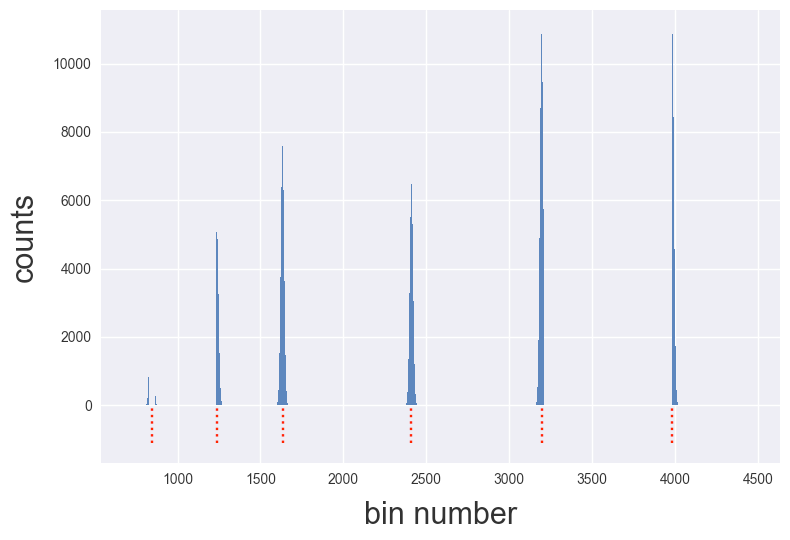
\includegraphics[width=\textwidth]{time_calibration_counts_over_bin.png}
\caption{Peaks in TDC bin number due to pulses sent with varying known time-delays.
The red dotted lines show the estimated peak positions. A gaussian filter has been applied to group the TDC values from each peak together.}
\label{fig:time_calibration_data}
\end{subfigure}
\hfill
\begin{subfigure}[t]{0.45\textwidth}
    \centering
    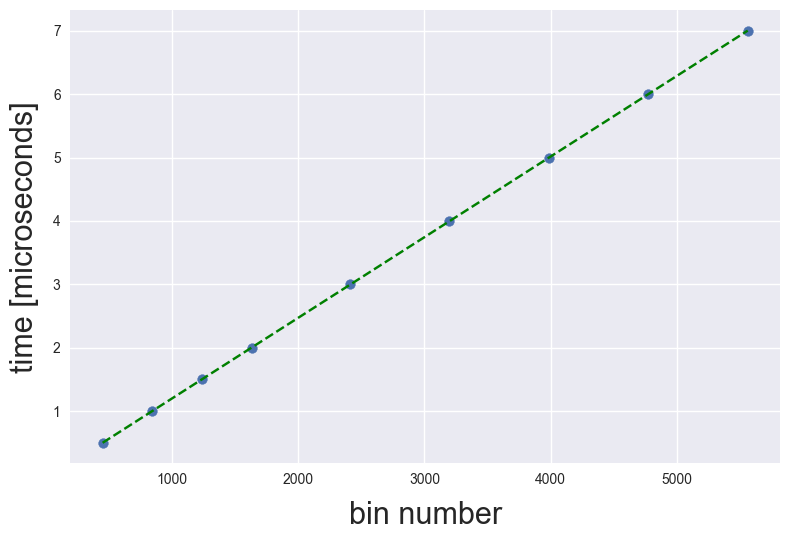
\includegraphics[width=\textwidth]{time_calibration_fit.png}
    \caption{Linear fit of the pulse time-differences to TDC bin number.}
    \label{fig:time_calibration_fit}
\end{subfigure}
\caption{}
\label{fig:time_calibration}
\end{figure}


\subsection{Fit function}

The fit function used to find the muon and pion lifetime in this report is

\begin{equation}\label{eq:fit_function}
\left[N_0 \left(e_p^{-\frac{t_s}{t_{\mu}}} - e_p^{-\frac{t_s}{t_{\pi}}}\right)\right]
* \left[\frac{1}{\sigma\sqrt{2\pi}}e^{-\frac{t_s^2}{2p_1^2}}\right]
,\end{equation}
where \(e_p^x = \begin{cases}
0 & \textnormal{if }x < 0 \\
e^x & \textnormal{else}
\end{cases}\) is used to model the decay function of the particles since there are no decays for values of \(x=t<0\).
The parameter \(t_s = t - t_0\), where \(t_0\) is the time shift (time until the first of the two pulses we record from our data),
 The symbol \(*\) is the convolution operator. The convolution with the gaussian factor on the right hand side of Equation \ref{eq:fit_function} has the effect of blurring the fit function to account for the finite resolution of the time signals from our experiment. 

The real data has a constant background that would need to be modeled in the fit, but we are able to subtract that background by taking the mean of the first few bins below \(t = t_0\), since this region should contain data from only that constant background.

We anticipated the need to model a hadronic background peak around \(t=t_0\) as well by adding another gaussian term. However, we did not see this peak in our data, and adding the term to our fit did not improve the reduced chi-squared (\(\chi_\nu^2\)) value we achieved. It did however reduce the stability of the fit, so it was omitted.  


\subsubsection{Reduced chi-squared}
The \(\chi_\nu^2\) value used to compare fits was calculated as
\[
\chi_\nu^2 = \frac{1}{\nu}\sum_i^N\frac{(O_i - F_i)^2}{F_i}
\]
where \(O_i\) is the observed value at a histogram bin \(i\), and \(F_i\) is the fitted value at that bin.
\(F_i\) was modified to be \(F_i \to \max(F_i,  1)\) to account for \(F_i=0\) values in the denominator.
\(\nu\) is the number of degrees of freedom: the number of bins minus the number of parameters in the fit.

The \(\chi_\nu\) value as we have defined it may not suitable as an absolute measure of the goodness of fit by via a chi-squared test, since after subtracting the constant background term, we have significant levels of background noise not modelled by the \(F_i \approx \sqrt{\sigma_i}\) factor. It may be possible to replace the \(F_i\) in the denominator with a factor that incorporates both the histogram uncertainty and the background noise uncertainty, but for this report, we only used the \(\chi_\nu^2\) value as a relative measure of goodness of fit between fit function, which was a task it was still well suited for.

\subsubsection{Minimization technique}
A global minimization technique was used to fit the parameters to the data. We used the \verb|scipy.optimize.dual_annealing| function, which used separate annealing methods to search for global minima and to optimize the parameters in a minima once found~\cite{scipy_dual_annealing}.

The bounds for this method were set to
\[
\begin{array}{c|c|c}
p1 \in (0,  100) & t_0 \in (0, 5\times 10^{-6}) & N_0 \in (0, 100)\\
t_\mu \in (0, 1\times 10^{-5}) & t_\pi \in (0, 1\times 10^{-5}) &
\end{array}
\]
All these bounds were estimated by looking at the histogrammed data, or by seeing if the fit parameters often reached a boundary in the minimization process.

\subsubsection{Fit parameter uncertainty}
The uncertainty on the fit parameters follows the same technique as the\\
\verb|scipy.optimize.leastsq| method~\cite{scipy_hessian}.

The hessian \(H\) of the sum of residuals squared is numerically computed at the minima found by the fit function, The covariance matrix is then computed as
\begin{equation}
C = H^{-1}\sigma_r^2
\end{equation}
where \(\sigma_r^2\) is the variance of the residuals.
The parameter uncertainties are then taken as
\begin{equation}
    \sigma_p = \sqrt{\textnormal{diag}(C)}
\end{equation}
where the square-root function is applied piecewise.

\subsubsection{Simulated data}
Prior to obtaining the experimental data, simulated data was produced in order to test our fitting process whilst also giving a comparison for the final results. The data was simulated by sampling the \verb|np.random.exponential| function for the lifetime of muon and the pion, then adding the lifetimes together.

100,000 of these total lifetimes were simulated, then placed in a histogram (similar to how the TDC discretizes the data). Other factors were included to make the simulated data set resemble what was expected from the real data. Namely, a constant time shift of $1.75 \cdot 10^{-6}$ seconds was used as this was also included in the acquisition of the real data. Additionally, a uniform background was included using the \verb|np.random.uniform| function and a gaussian blur was applied using the function \verb|scipy.ndimage.gaussian_filter1d|.

\begin{figure}[h]
\centering
\begin{subfigure}[t]{0.45\textwidth}
\centering
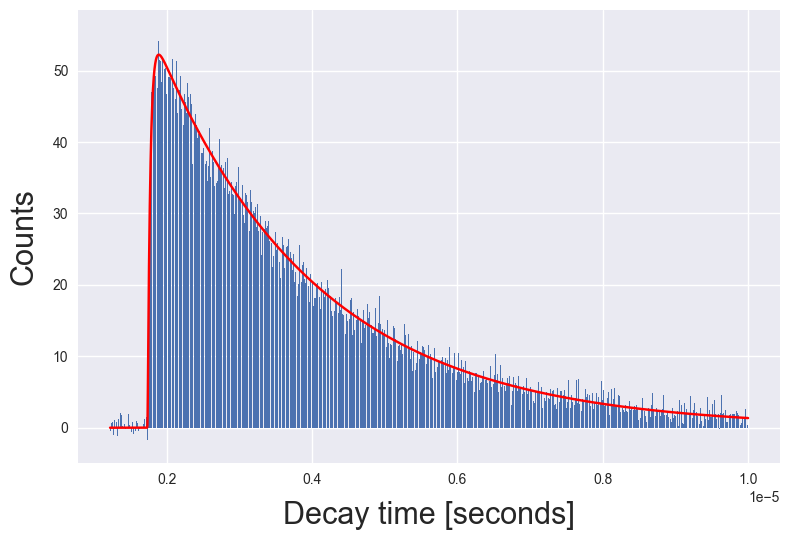
\includegraphics[width=\textwidth]{simulated_histogram.png}
\caption{Simulated data with constant background subtracted.}
\label{fig:simulated_data}
\end{subfigure}
\hfill
\begin{subfigure}[t]{0.45\textwidth}
    \centering
    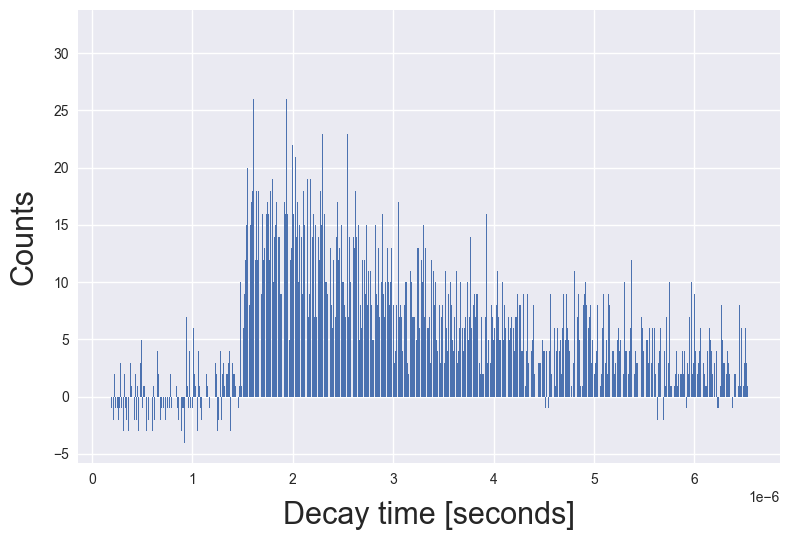
\includegraphics[width=\textwidth]{experimental_histogram.png}
    \caption{Experimental data with edges cut to match simulated data, and constant background subtracted.}
    \label{fig:experimental_data}
\end{subfigure}
\caption{}
\label{fig:data}
\end{figure}



The simulated data gave us a good basis in which we could understand the general shape to expect of the experimental data as well as the scales we are working on, especially concerning the time axis. 

With the true value of the muon (pion) set in our fit as \(t_\mu=2.1969811 \times 10^{-6}\) (\(t_\pi=2.6033 \times 10^{-8}\))~\cite{Literature Values}, and the results of the fit given as \(\hat t_\mu\) (\(\hat t_\pi\)).

The fit in Figure~\ref{fig:simulated_data} gives
\begin{align}
(\hat t_\mu - t_\mu) \pm \delta \hat t_\mu
&= (0.01 \pm 0.30) \times 10^{-6}\\
(\hat t_\pi - t_\pi) \pm \delta \hat t_\pi
&= (1.0827 \pm 73) \times 10^{-8}
\end{align}

Therefore, both lifetimes agree with the parameters they were set to within the uncertainties of the fit. This gave us confidence to use this method on the experimental data.

\subsubsection{Experimental data}
After producing and analyzing the simulated data, we obtained the data from the experiment.

The real data followed a similar shape to our simulated data, except that the real data contained peaks on the left and right hand edges of the histogram accumulated from the overflow of the TDC (Fig. \ref{fig:full_experimental_histogram}). These peaks were cut before fitting.

\begin{figure}
    \centering
    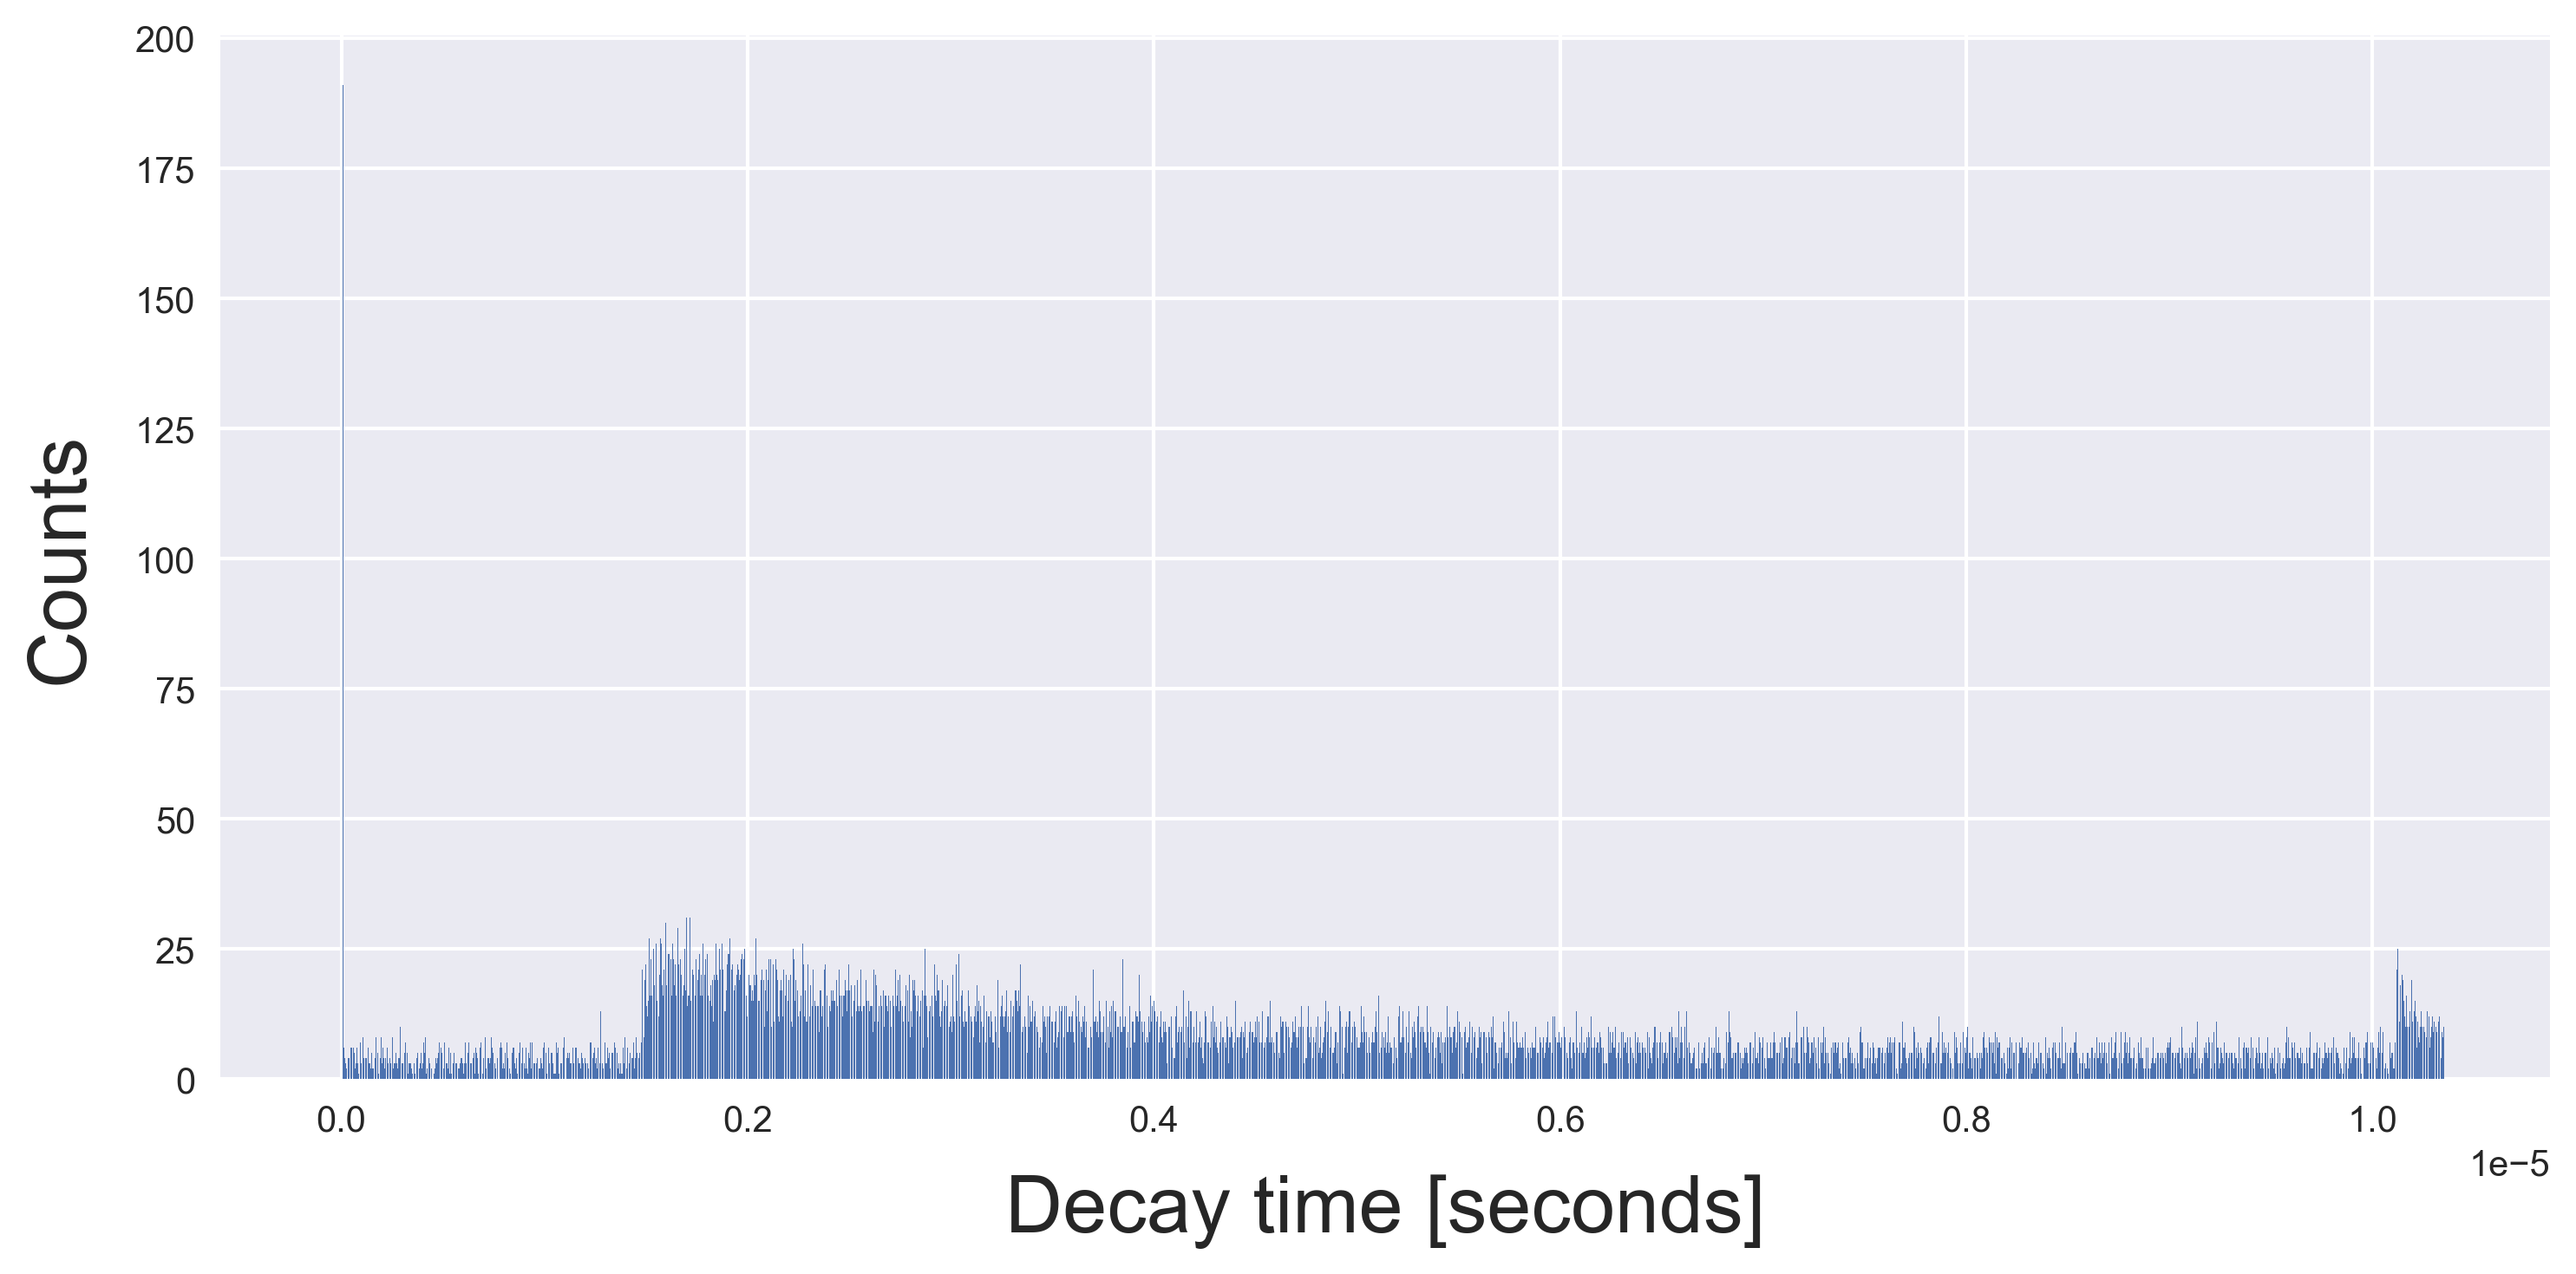
\includegraphics[width=1\linewidth]{full_experimental_histogram.png}
    \caption{The full range of the experimental histogram. Without the constant backgound subtracted and without the edges clipped.}
    \label{fig:full_experimental_histogram}
\end{figure}



\section{Results and Conclusion}
\subsection{Results }
The plot of the experimental data has a similar shape compared to the simulated one,
confirming the nature of the measured data is correct. Achieving this results was particularly valuable, as a significant amount of time had been lost, duo to troubleshooting a setup error that led to invalid data. However the accuracy of the data still varies quite a lot . 
The mean lifetime for a pion is $(2.6033 \pm 0.0005) \cdot 10^{-8} \text{ s}$ and for a muon $(2.1969811 \pm 0.0000022)\cdot 10^{-6} \text{ s} $, according to the particle data group (PDG)~\cite{Literature Values}. The results of the measurements along with their uncertainties are listed in \autoref{tab: Measurment results}.



\begin{table}[ht!]
\centering
\begin{tabular}{|c|c|c|c|c|}
\hline
&\multicolumn{2}{|c|}{\textbf{Pion [$10^{-8}$s]}} 
&\multicolumn{2}{|c|}{\textbf{Muon [$10^{-6}$s]}} \\
\hline
\textbf{Measurement} & \textbf{lifetime} & \textbf{fit uncertainty} & \textbf{lifetime} & \textbf{fit uncertainty}  \\
\hline
1 & 4.32596 & 66.6032  & 2.17728 & 1.92041  \\
2 & 0.315238 & 45.3617  & 2.24811 & 1.02218 \\
3 & 75.001 & NaN & 0.818083 & NaN \\
\hline
\end{tabular}
    \caption{The measurement results from all 3 measurements with their uncertainties.}
    \label{tab: Measurment results}
\end{table}

While normal discriminators weres used for the first and second measurement, a constant fraction discriminator was used for the third. The theory predicts a better result with the CFD, but in this experiment the normal discriminators are more accurate. While the reason for this is unknown, it is probably due to and old and maybe defective CFD

The bin uncertainty from the time calibration is on the order of $10^{-9}$, and can therefore be neglected considering the smallest fit uncertainty is of order $10^{-7}$. This would only have an effect on the combined uncertainty at the 6th significant digit (of the smallest uncertainty) since 
\[
\sqrt{(10^{-7})^2 + (10^{-9})^2} - 10^{-7} \approx 5 \times 10^{-12}
\]
Following a similar reasoning, the uncertainties given by the PDG can be ignored in the determination of the final agreement, as they are both of order $10^{-12}$.

Therefore, we can state the agreements as shown in \autoref{tab:measurement_agreement}.

\begin{table}[ht!]
\centering
\begin{tabular}{|c|c|c|c|c|}
\hline
&\multicolumn{2}{|c|}{\textbf{Pion [$10^{-8}$s]}} 
&\multicolumn{2}{|c|}{\textbf{Muon [$10^{-6}$s]}} \\
\hline
\textbf{Measurement} & \(\hat t_\pi - t_\pi\) & \(\delta \hat t_\pi\) & \(\hat t_\mu - t_\mu\) & \(\delta \hat t_\mu\) \\
\hline
1 & 1.7 & 66&-0.02&1.92 \\
2 &-2.3&45&0.05&1.02 \\
3 &72.3977&NaN&-1.37&NaN \\
\hline
\end{tabular}
    \caption{The agreement of the measurements.}
    \label{tab:measurement_agreement}
\end{table}

We see that the values for the muon and the pion lifetime agree with literature values within their uncertainties for measurments 1 and 2, and that the agreement for measurement 3 cannot be determined, since the uncertainties for that run did not converge. 



\subsection{General problems and possible errors}
The time calibration was done really accurately with the linear fit precisely hitting the measurement points well. Therefore it can be neglected, and the focus should be in finding the larger error sources. \\
For instance, there were unknown problems with one of the discriminators, and also, because
the main beam line was turned off multiple times the day before the planned data collection, there was less data collected than planned. 
This not only resulted in a less representative evaluation of the data, but also in a noisier spectrum. Random coincidences, meaning unrelated signals mimicking decays, or hadronic interactions in the detector itself are much harder to identify and subtract with limited statistics. \\
For that reason, having more beam time to collect data would help to improve the values in any future attempts by reducing the background noise and lowering the statistical uncertainties. \\ Furthermore a exponential function had to be coded in python to fit to the data and although all relevant fit parameters were included, the limited data did not allow to determinate the parameters with absolute accuracy. A more thorough calibration and a refined statistical analysis could help improve the function and resulting values.




\subsection{Muons vs. Pions}
The value received for the muon is significantly closer to the literary vale than the one of the pion. This has a few possible reasons: \\
To begin with, the pion's lifetime is of the same order of magnitude as the time resolution of the used electronics. According to studies conducted at CERN~\cite{Scintillator timing resolution} the timing resolution of a modern scintillator is in the realms of picoseconds. However, for older equipment and electronics as the ones used in this experiment, this is not yet achievable. This limitation in equipment quality leads to a broadening of the measured decay-time spectrum (smearing).
This distorts the exponential shape particularly at short times and leads to a time resolution in the order of \SI{1}{ns}. This affects the accuracy of the pion measurement significantly more strongly, since its lifetime is of the same order of magnitude as the timing resolution. \\
In addition, from the theory one would expect a sharp peak from hadronic interactions at the beginning of the measurement. Since it was not able to separate this in the received data, it distorts the measurements of shorter lifetimes, in this case, the pions.





\subsection{Summary}
The experiment was successful in determining a mean lifetime for pions and muons. 
This experiment demonstrated the procedure behind setting up and conducting an experiment using a proton beam, including which safety measures and electronics are used and the calculation of the lifetime of a particle by time distribution. Since the results are in the same order of magnitude but not within the error tolerance of the literature values, it would make sense to collect more data and further improve the analysis function if the experiment is repeated.











\newpage

\begin{thebibliography}{99}

\bibitem[1]{Mittlere Lebensdauer} 
Rhetos Lexikon der Physik. (2025). \textit{Mittlere Lebensdauer}. 
Retrieved from \url{https://www.rhetos.de/html/lex/mittlere_lebensdauer.htm} (accessed 12 Sept 2025).

\bibitem[2]{Lebensdauer} 
Wikipedia. (2025). \textit{Lebensdauer (Quantenphysik)}. 
Retrieved from \url{https://de.wikipedia.org/wiki/Lebensdauer_(Quantenphysik)} (accessed 12 Sept 2025).

\bibitem[3]{Povh}
Povh, B., Rith, K., Scholz, C., Zetsche, F., \& Rodejohann, W. (2014). \textit{Particles and nuclei: An introduction to the physical concepts}. Springer. 

\bibitem[4]{PPE at PSI}
Caminada, L., Schmidt-Wellenberg, P., \& Steinkamp, O. (2025). \textit{Particle Physics Experiment at PSI (PHY462)}. Lecture material.

\bibitem[5]{muon decay}
Fetscher, W. (2021). \textit{Muon decay}. SciPost Physics Proceedings 5, 006.  
Retrieved from \url{https://scipost.org/SciPostPhysProc.5.006/pdf} (accessed 12 Sept 2025).

\bibitem[6]{PSI cyclotron}
Paul Scherrer Institute (PSI). (2025). \textit{The Ring Cyclotron}.  
Retrieved from \url{https://www.psi.ch/en/cas/ring} (accessed 12 Sept 2025).

\bibitem[7]{PSI PiM1}
Paul Scherrer Institute (PSI). (2025). \textit{Scintillator Panels, PiM1 Beamline}.  
Retrieved from \url{https://www.psi.ch/en/sbl/pim1-beamline} (accessed 12 Sept 2025).

\bibitem[8]{Scint}
CERN. (2025). \textit{Plastic scintillators}.  
Retrieved from \url{https://alpha.web.cern.ch/science/plastic-scintillators} (accessed 29 Aug 2025).

\bibitem[9]{CFD}
Wikipedia. (2025). \textit{Constant fraction discriminator}.  
Retrieved from \url{https://en.wikipedia.org/wiki/Constant_fraction_discriminator} (accessed 11 Sept 2025).

\bibitem[10]{Literature Values}
Navas, S. et al. (Particle Data Group). (2024). \textit{Review of Particle Physics}. Phys. Rev. D 110, 030001.  
Retrieved from \url{https://pdg.lbl.gov/2025/tables/contents_tables.html} (accessed 12 Sept 2025).

\bibitem[11]{Scintillator timing resolution}
Alici, A., et al. (2018). \textit{Scintillator timing resolution}. JINST 13, P09012.  
DOI: 10.1088/1748-0221/13/09/P09012. Retrieved from \url{https://iopscience.iop.org/article/10.1088/1748-0221/13/09/P09012/pdf} (accessed 12 Sept 2025).


\bibitem[12]{scipy_dual_annealing}
Pauli Virtanen, Ralf Gommers, Travis E. Oliphant, Matt Haberland, Tyler Reddy, David Cournapeau, Evgeni Burovski, Pearu Peterson, Warren Weckesser, Jonathan Bright, Stéfan J. van der Walt, Matthew Brett, Joshua Wilson, K. Jarrod Millman, Nikolay Mayorov, Andrew R. J. Nelson, Eric Jones, Robert Kern, Eric Larson, CJ Carey, İlhan Polat, Yu Feng, Eric W. Moore, Jake VanderPlas, Denis Laxalde, Josef Perktold, Robert Cimrman, Ian Henriksen, E.A. Quintero, Charles R Harris, Anne M. Archibald, Antônio H. Ribeiro, Fabian Pedregosa, Paul van Mulbregt, and SciPy 1.0 Contributors. (2020) SciPy 1.0: Fundamental Algorithms for Scientific Computing in Python. Nature Methods, 17(3), 261-272. DOI: 10.1038/s41592-019-0686-2. \textit{Ccipy leastsq covariance estimation.}
Retrieved from 
\url{https://docs.scipy.org/doc/scipy/reference/generated/scipy.optimize.dual_annealing.html} (accessed 15 Sept 2025)

\bibitem[13]{scipy_hessian}
Pauli Virtanen, Ralf Gommers, Travis E. Oliphant, Matt Haberland, Tyler Reddy, David Cournapeau, Evgeni Burovski, Pearu Peterson, Warren Weckesser, Jonathan Bright, Stéfan J. van der Walt, Matthew Brett, Joshua Wilson, K. Jarrod Millman, Nikolay Mayorov, Andrew R. J. Nelson, Eric Jones, Robert Kern, Eric Larson, CJ Carey, İlhan Polat, Yu Feng, Eric W. Moore, Jake VanderPlas, Denis Laxalde, Josef Perktold, Robert Cimrman, Ian Henriksen, E.A. Quintero, Charles R Harris, Anne M. Archibald, Antônio H. Ribeiro, Fabian Pedregosa, Paul van Mulbregt, and SciPy 1.0 Contributors. (2020) SciPy 1.0: Fundamental Algorithms for Scientific Computing in Python. Nature Methods, 17(3), 261-272. DOI: 10.1038/s41592-019-0686-2. \textit{Ccipy leastsq covariance estimation.}
Retrieved from \url{https://github.com/scipy/scipy/blob/b1296b9b4393e251511fe8fdd3e58c22a1124899/scipy/optimize/_minpack_py.py#L349-L355} (accessed 15 Sept 2025)

\end{thebibliography}


\end{document}
